%----------------------------------------------------------------------
% Main document for the thesis template
%----------------------------------------------------------------------
\documentclass[
    ieee,      % Bibliography style: ieee, wmaainf
    bachelor,  % Type of thesis: master, bachelor, report
    german,    % Language: german, english
    singlepage % Cover Layout: singlepage, doublepage
]{ohm}
% \nocite{*} % nur zu Testzwecken - bleibt deaktiviert (nur zitierte Quellen im Verzeichnis)
\usepackage{booktabs}
\usepackage{csquotes}
\usepackage{tikz}
\usepackage{qrcode}
\usepackage{pgfplots}
\pgfplotsset{compat=1.18}
\usetikzlibrary{positioning, arrows.meta, fit, backgrounds}
%----------------------------------------------------------------------
% Verzeichnisse im Inhaltsverzeichnis auffuehren.
% Reihenfolge: \clearpage (frische Seite) -> \phantomsection (Hyperref-Anker)
% -> \addcontentsline (Eintrag mit korrekter Seitenzahl) -> Verzeichnis.
%----------------------------------------------------------------------
\newcommand{\addverzeichnis}[1]{%
  \clearpage
  \phantomsection
  \addcontentsline{toc}{chapter}{#1}%
}
%----------------------------------------------------------------------
% Meta data section
%----------------------------------------------------------------------
\title{Szenenverständnis und -manipulation in immersiven Umgebungen mittels Künstlicher Intelligenz}
\author{Sandro Jäger}
\studentid{3683886}
\date{\today}
%----------------------------------------------------------------------
\examiner{Prof.\,Dr.\,Uwe Wienkop}
\examiner{Louis Burk}
%----------------------------------------------------------------------
% Schlagwoerter (erscheinen in der Kurzdarstellung-Sektion und in den PDF-Metadaten)
\keyword{Szenenrepräsentation}
\keyword{Immersive Umgebungen}
\keyword{Multimodale Agenten}
\keyword{Lokale Sprachmodelle}
\keyword{Vision-Language-Modelle}
%----------------------------------------------------------------------
\repository{https://git.informatik.fh-nuernberg.de/jobboerse/forschung/bachelorarbeiten/bachelorarbeit-sandro-jaeger}
%----------------------------------------------------------------------
% Englischer Abstract nur bei englischer Arbeit noetig -> hier (deutsch) leer.
\begin{abstract}
\end{abstract}
%----------------------------------------------------------------------
\begin{kurzdarstellung}
    Damit ein KI-Agent eine dreidimensionale Szene über natürliche Sprache verändern kann, muss ihm die Szene zuerst in einer Form vorliegen, die er verarbeiten kann.
    Grundsätzlich gibt es dafür zwei Wege, zum einen eine strukturelle Beschreibung als exakte Daten und zum anderen eine visuelle Beschreibung über ein gerendertes Bild.
    Für selbst gehostete Modelle geringer Größe fehlte bisher ein systematischer Vergleich dieser beiden Formen.

    Die vorliegende Arbeit untersucht deshalb, welchen Einfluss die Repräsentationsform auf den Ausführungserfolg der Szenenmanipulation hat und ob sich eine Kombination beider Formen gezielt gestalten lässt.
    Dafür wurde ein prototypisches System entwickelt, das dieselbe Szene strukturell, visuell und hybrid bereitstellt und fünf daraus abgeleitete Varianten unter gleichen Bedingungen an dreizehn kontrolliert aufgebauten Szenarien vergleicht.
    Gemessen wurde am Desktop.

    Im Vergleich zeigt sich, dass keine Form über alle Aufgaben hinweg überlegen ist und beide Formen jeweils einen Bereich abdecken, den die andere nicht erreicht.
    Eine naive Kombination vereint diese Stärken nicht von selbst.
    Während eine Priorisierung einer Schicht das Gewicht nur verschiebt, bringt eine klare Trennung der Zuständigkeiten beide Schichten auf dem untersuchten Szenarioset zusammen.
    Ein Demonstrator überträgt diese Variante in eine immersive Umgebung und zeigt, dass die gesamte Kette funktioniert.
\end{kurzdarstellung}
%----------------------------------------------------------------------
\begin{acknowledgements}
    Mein Dank gilt Prof.\,Dr.\,Uwe Wienkop und Louis Burk für die Betreuung dieser Arbeit und für die hilfreichen Rückmeldungen im Verlauf.
    Dem Institut für angewandte Informatik danke ich für die Möglichkeit, diese Arbeit dort anzufertigen, sowie für die bereitgestellte Hardware, ohne die der lokale Betrieb der Modelle nicht möglich gewesen wäre.
    Ein besonderer Dank gilt schließlich meinem Bruder und meinen Eltern für ihre Unterstützung während des Studiums.
\end{acknowledgements}
%----------------------------------------------------------------------
% Import glossary and acronym definitions
%----------------------------------------------------------------------
%----------------------------------------------------------------------
% Abkuerzungs- und Glossareintraege
%----------------------------------------------------------------------
\makenoidxglossaries
%----------------------------------------------------------------------
% --- Abkuerzungen (Abkuerzungsverzeichnis) ---
%----------------------------------------------------------------------
\newacronym{ki}{KI}{Künstliche Intelligenz}
\newacronym{llm}{LLM}{Large Language Model, großes Sprachmodell}
\newacronym{vlm}{VLM}{Vision-Language Model, Sprach-Bild-Modell}
\newacronym{mcp}{MCP}{Model Context Protocol}
\newacronym{som}{SoM}{Set-of-Mark}
\newacronym{vr}{VR}{Virtual Reality, virtuelle Realität}
\newacronym{mr}{MR}{Mixed Reality, gemischte Realität}
\newacronym{vpn}{VPN}{Virtual Private Network, virtuelles privates Netz}
\newacronym{json}{JSON}{JavaScript Object Notation}
\newacronym{api}{API}{Application Programming Interface, Programmierschnittstelle}
\newacronym{gpu}{GPU}{Graphics Processing Unit, Grafikprozessor}
\newacronym{vram}{VRAM}{Video Random Access Memory, Grafikspeicher}
\newacronym{stt}{STT}{Speech-to-Text, Spracherkennung}
\newacronym{rq}{RQ}{Research Question, Forschungsfrage}
\newacronym{fa}{FA}{funktionale Anforderung}
\newacronym{nfa}{NFA}{nicht-funktionale Anforderung}
\newacronym{es}{ES}{Execution Success, Ausführungserfolg}
%----------------------------------------------------------------------
% --- Glossarbegriffe ---
%----------------------------------------------------------------------
\newglossaryentry{lokaler-betrieb}{
  name={lokaler Betrieb},
  description={Selbst gehosteter Betrieb der Modelle ohne Cloud-Dienst,
  siehe Abschnitt~\ref{sec:ein-motivation}}
}
\newglossaryentry{strukturelle-repraesentation}{
  name={strukturelle Repräsentation},
  description={Bereitstellung der Szene als exakte Laufzeitdaten der Engine
  (Objekt-ids, Typen, Positionen, Größen, Farben, Kamerapose) in textueller
  Form, hier als JSON}
}
\newglossaryentry{visuelle-repraesentation}{
  name={visuelle Repräsentation},
  description={Bereitstellung der Szene über eine von einem Sprach-Bild-Modell
  erzeugte natürlichsprachliche Beschreibung der gerenderten, mit
  Set-of-Mark-Markern versehenen Ansicht, siehe
  Abschnitt~\ref{sec:grundlagen-modelle}}
}
\newglossaryentry{naive-hybride-repraesentation}{
  name={naive hybride Repräsentation},
  description={Kombination aus struktureller und visueller Schicht ohne
  verbindliche Instruktion zur Zuständigkeit der beiden Quellen}
}
\newglossaryentry{priorisierende-hybride-repraesentation}{
  name={priorisierende hybride Repräsentation},
  description={Hybride Repräsentation mit vorangestellter visueller
  Beschreibung, die als maßgeblich für das Aussehen deklariert wird}
}
\newglossaryentry{kompetenzgetrennte-hybride-repraesentation}{
  name={kompetenzgetrennte hybride Repräsentation},
  description={Hybride Repräsentation mit expliziter Aufgabenteilung: die
  visuelle Beschreibung bestimmt, welches Objekt gemeint ist, die
  strukturelle Schicht liefert alle numerischen Werte}
}
\newglossaryentry{kennungssystem}{
  name={gemeinsames Kennungssystem},
  description={Einheitliche Objektkennungen, über die alle
  Repräsentationsvarianten Objekte ansprechen; die visuelle Variante ist über
  ihre Bildmarken an dieselben Kennungen gebunden}
}
\newglossaryentry{grounding}{
  name={Grounding},
  description={Auflösung einer sprachlichen Referenz auf ein konkretes
  Szenenobjekt}
}
\newglossaryentry{folgezustand}{
  name={Folgezustand},
  description={Tatsächlicher Zustand der Szene nach einer Manipulation, aus
  dem der Ausführungserfolg unabhängig von der Selbstauskunft des Agenten
  bestimmt wird}
}
\newglossaryentry{referenztyp}{
  name={Referenztyp},
  description={Art, in der ein natürlichsprachlicher Befehl auf ein Objekt
  verweist, etwa über eine Kennung, ein Attribut, eine räumliche Relation,
  eine rein sichtbare Eigenschaft oder ein verdecktes Objekt}
}

%----------------------------------------------------------------------
% Begin document
%----------------------------------------------------------------------
\begin{document}
%----------------------------------------------------------------------
% \frontmatter -- roman page numbers (i, ii, iii, ...)
%----------------------------------------------------------------------
\frontmatter
%----------------------------------------------------------------------
% Cover pages
%----------------------------------------------------------------------
\maketitle
%----------------------------------------------------------------------
% Die Selbststaendigkeitserklaerung (SB_0009) wird nicht im Dokument
% benoetigt und daher hier bewusst nicht eingebunden.
%----------------------------------------------------------------------
\makeabstract          % Kurzdarstellung + Schlagwoerter
\makeacknowledgements  % Danksagung
\maketableofcontents
%----------------------------------------------------------------------
% Verzeichnisse: vollstaendig VOR Kapitel 1 und im Inhaltsverzeichnis
% aufgefuehrt. \addverzeichnis setzt den TOC-Eintrag samt Hyperref-Anker.
%----------------------------------------------------------------------
\glsaddall  % noidx-Glossare listen nur benutzte Eintraege -> alle aufnehmen
\addverzeichnis{Abkürzungsverzeichnis}
\makeacronyms
\addverzeichnis{\listfigurename}
\listoffigures
\addverzeichnis{\listtablename}
\listoftables
\addverzeichnis{\listoflistingscaption}
\listoflistings
%----------------------------------------------------------------------
% \mainmatter -- arabic page numbers, restarting at 1
%----------------------------------------------------------------------
\mainmatter
%----------------------------------------------------------------------
% ============================================================
% KAPITEL 1 — EINLEITUNG
% ============================================================

\chapter{Einleitung}
\label{ch:einleitung}

% ------------------------------------------------------------
\section{Motivation und Problemstellung}
\label{sec:ein-motivation}

Ein Nutzer steht in einer virtuellen Szene und gibt einen einfachen Befehl: \enquote{Heb den gestreiften Würfel an.}
Für einen Menschen ist das ziemlich simpel.
Ein KI-Agent muss dagegen zuerst wissen, wie die Szene aussieht, und diese Information muss ihm in einer Form vorliegen, die er auch verarbeiten kann.

Grundsätzlich gibt es dafür zwei Wege.
Die Szene lässt sich strukturell beschreiben, also als exakte Daten über die Objekte mit ihren Typen, Positionen und Größen, oder visuell als gerendertes Bild, das ein visuelles Modell interpretiert.
Beide Wege haben Stärken und blinde Flecken.
Die strukturellen Daten kennen jede Koordinate, über das Aussehen eines Objekts sagen sie nichts, und beim Bild ist es andersherum.

Der gestreifte Würfel aus dem Beispiel zeigt den ersten blinden Fleck.
Da das Streifenmuster in keinen strukturellen Daten steht, lässt sich der Würfel nur über das Bild bestimmen.
Ebenso gibt es den umgekehrten Fall.
Steht ein Objekt hinter einem anderen, taucht es im Bild überhaupt nicht auf, obwohl es in den strukturellen Daten vollständig verzeichnet ist.
Ein Befehl, der sich auf ein solches Objekt bezieht, lässt sich nur über die Struktur auflösen.

Wer einen solchen Agenten entwickelt, muss deshalb früh entscheiden, in welcher Form er ihm die Szene bereitstellt und ob sich beide Wege sinnvoll kombinieren lassen.
Besonders wichtig ist diese Entscheidung in immersiven Umgebungen, in denen Nutzer über natürliche Sprache mit einer Szene interagieren.
Dort bieten sich lokal betreibbare Modelle an, vor allem wegen Datenschutz, Latenz und Offline-Fähigkeit, und für solche Modelle gibt es bisher keinen systematischen Vergleich der beiden Wege.

Mit \emph{lokal} ist in dieser Arbeit durchgängig ein selbst gehosteter Betrieb auf eigener Hardware ohne Cloud-Dienst gemeint, bei dem keine Szenen- oder Sprachdaten das eigene Netz verlassen.
Auf dem Endgerät selbst müssen die Modelle dafür nicht rechnen.
Sowohl in der Messung als auch im Demonstrator laufen die Modelle auf einem Arbeitsplatzrechner, den die Brille im Demonstrator über eine Netzverbindung innerhalb des Institutsnetzes erreicht (Abschnitt~\ref{sec:impl-demonstrator}).


% ------------------------------------------------------------
\section{Relevanz}
\label{sec:ein-relevanz}

Die Wahl der Repräsentationsform entscheidet mit darüber, welche sprachlichen Anweisungen ein Agent überhaupt zuverlässig umsetzen kann.
Fehlt in einer Repräsentation eine ganze Klasse von Referenzen, scheitern die zugehörigen Befehle, egal wie gut der Agent ansonsten arbeitet.

Große, cloudbasierte Modelle können eine schwache Repräsentation teilweise durch ihre Größe ausgleichen.
Bei kleinen, lokal betriebenen Modellen ist das kaum möglich, weshalb die Repräsentation hier eine deutlich größere Rolle spielt.
Die Entscheidung über die Repräsentationsform fällt früh im Entwurf, hat weitreichende Folgen und wird bislang ohne belastbare Grundlage getroffen.

Darüber hinaus betrifft die Frage auch ein allgemeineres Problem.
Sobald ein Agent strukturierte und visuelle Information gemeinsam verarbeitet, stellt sich die Frage, ob sich beide Informationsarten ergänzen oder ob eine die andere verdrängt.
Auch über den hier untersuchten Anwendungsfall hinaus ist diese Frage noch offen~\cite{deng2025, wu2025}.


% ------------------------------------------------------------
\section{Zielsetzung und Forschungsfragen}
\label{sec:ein-ziele}

Diese Arbeit untersucht, welche Repräsentationsform einen lokal betriebenen Agenten bei der natürlichsprachlichen Szenenmanipulation am zuverlässigsten unterstützt.
Dafür werden zwei Forschungsfragen gestellt.

\begin{quote}
\textbf{Forschungsfrage~1 (RQ1).}
Welchen Einfluss hat die Form der Szenenrepräsentation, strukturell, visuell oder hybrid, auf den Ausführungserfolg der natürlichsprachlichen Szenenmanipulation durch einen lokal betriebenen Agenten, und zwar aufgeschlüsselt nach der Art der sprachlichen Referenz?

\vspace{6pt}
\textbf{Forschungsfrage~2 (RQ2).}
Lässt sich das Zusammenspiel der strukturellen und der visuellen Schicht allein durch die Gestaltung der Instruktion so steuern, dass die hybride Repräsentation die Stärken beider Schichten vereint?
\end{quote}

Die Stärken beider Schichten gelten für RQ2 dann als vereint, wenn eine gestaltete Instruktion dort deutlich besser abschneidet, wo die bloße Kombination beider Schichten scheitert, und in den übrigen Aufgaben nicht schlechter wird.

Gemessen wird in beiden Fällen ausschließlich der Ausführungserfolg.
Er wird für jeden Lauf binär aus dem tatsächlichen Szenenzustand bestimmt.
Ein Lauf ist nur erfolgreich, wenn das gemeinte Objekt betroffen ist und das geforderte Ergebnis eintritt, bei Positionsaufgaben innerhalb einer festen Toleranz.
Ein kontinuierlicher Lagefehler gehört nicht zur Zielgröße und wird nicht berichtet.
Die genaue Definition folgt in Abschnitt~\ref{sec:eval-metrics}.

Untersucht wird ein lokales Modellpaar in kontrolliert aufgebauten Szenen, gemessen wird am Desktop.
Zusätzlich entsteht ein Demonstrator, der die zuverlässigste Variante in die immersive Zielumgebung überträgt und die praktische Machbarkeit zeigen soll, ohne eine eigene Forschungsfrage zu beantworten.


% ------------------------------------------------------------
\section{Methodisches Vorgehen}
\label{sec:ein-vorgehen}

Die Arbeit verfolgt einen empirischen Ansatz.
Grundlage ist ein prototypisches System, das dieselbe Szene in allen drei Repräsentationsformen bereitstellt und über ein gemeinsames Interface manipulierbar macht.
Mit diesem System werden die Formen unter gleichen Bedingungen an kontrolliert aufgebauten Szenarien miteinander verglichen.
Ob eine Manipulation erfolgreich war, wird aus dem tatsächlichen Zustand der Szene bestimmt und nicht aus der Rückmeldung des Agenten, und jede Messung wird mehrfach wiederholt, um zufällige von belastbaren Unterschieden trennen zu können.

Daraus ergeben sich drei Beiträge, die in Abschnitt~\ref{sec:zus-beitrag} noch einmal aufgegriffen und eingeordnet werden.
Inhaltlich zeigt die Arbeit an einem kontrollierten Fall, dass sich strukturelle und visuelle Information nicht von selbst ergänzen und ihre Verbindung bewusst gestaltet werden muss.
Methodisch wird eine nach Referenztypen aufgeschlüsselte Auswertung eingeführt, die Zuständigkeiten der Repräsentationen sichtbar macht, die bei einem pauschalen Vergleich verborgen blieben.
Praktisch entsteht ein lauffähiger Demonstrator, der die gesamte Kette bis in die immersive Zielumgebung überträgt.


% ------------------------------------------------------------
\section{Aufbau der Arbeit}
\label{sec:ein-aufbau}

In Kapitel~\ref{ch:grundlagen} werden die für die Arbeit notwendigen Grundlagen dargestellt, die Arbeit in den Stand der Technik eingeordnet und die Forschungslücke abgeleitet.
Kapitel~\ref{ch:anforderungen} beschreibt, welche Anforderungen ein System erfüllen muss, um die Forschungsfragen beantworten zu können.
In Kapitel~\ref{ch:konzept} wird daraus das Lösungskonzept entwickelt, vor allem die drei Repräsentationsformen und die Entscheidungen, die einen fairen Vergleich ermöglichen.
Kapitel~\ref{ch:implementierung} beschreibt die technische Umsetzung, Kapitel~\ref{ch:evaluation} enthält den Vergleich und die Ergebnisse zu beiden Forschungsfragen.
Kapitel~\ref{ch:zusammenfassung} schließt mit einer Zusammenfassung und einem Ausblick.

% ============================================================
% KAPITEL 2 — GRUNDLAGEN UND STAND DER TECHNIK
% ============================================================

\chapter{Grundlagen und Stand der Technik}
\label{ch:grundlagen}

Dieses Kapitel führt zunächst die eingesetzten Modelle, das Agenten-Paradigma und die Formen der Szenenrepräsentation ein und ordnet die Arbeit anschließend in den Stand der Technik ein.


% ------------------------------------------------------------
\section{Große Sprach- und Sprach-Bild-Modelle}
\label{sec:grundlagen-modelle}

Die Arbeit setzt zwei Arten vortrainierter Modelle als Bausteine ein, die unverändert genutzt und nicht weiterentwickelt werden.

Ein großes Sprachmodell, im Folgenden als LLM (Large Language Model) bezeichnet, ist ein auf umfangreichen Textmengen trainiertes neuronales Modell, das zu einer Eingabe fortlaufend Text erzeugt.
Durch zusätzliches Training auf Instruktionen lässt es sich anweisen, eine Aufgabe zu bearbeiten, und gibt seine Antwort wiederum als Text aus.
In dieser Arbeit übernimmt ein LLM die Rolle des Agenten, der einen Befehl interpretiert und die passende Operation auswählt.
% CITATION: Grundlagenreferenz zu LLMs bzw. Instruction-Tuning ergaenzen (Survey/Lehrbuch).

Ein Sprach-Bild-Modell, im Folgenden als VLM (Vision-Language Model) bezeichnet, erweitert dieses Prinzip um eine visuelle Eingabe.
Es verarbeitet ein Bild zusammen mit einem Text und erzeugt daraus eine textuelle Antwort, etwa eine Beschreibung des Bildinhalts oder die Antwort auf eine Frage zum Bild.
In dieser Arbeit übernimmt ein VLM die visuelle Wahrnehmung der Szene.
% CITATION: Grundlagenreferenz zu VLMs ergaenzen (Survey).

Die beiden Modelle sind im hier untersuchten System nicht zu einem multimodalen Modell verschmolzen, sondern hintereinandergeschaltet.
Das Sprach-Bild-Modell erhält das gerenderte Bild und erzeugt daraus eine natürlichsprachliche Beschreibung.
Erst diese Beschreibung gelangt in den Kontext des Sprachmodells, das den Befehl deutet und die Operation wählt.
Das Modell, das die eigentliche Entscheidung trifft, sieht also zu keinem Zeitpunkt ein Bild.

Diese Eigenschaft des Aufbaus ist für die Deutung aller späteren Ergebnisse wichtig.
Was in dieser Arbeit \enquote{visuelle Repräsentation} heißt, ist streng genommen keine Bildeingabe, sondern die sprachliche Beschreibung eines Bildes.
Ist später von der Gewichtung der strukturellen gegenüber der visuellen Schicht die Rede, konkurrieren daher nicht Bild und Text im Inneren eines multimodalen Modells, sondern zwei Textquellen im Kontext eines reinen Sprachmodells: eine exakte, aber unvollständige Datenstruktur und eine reichhaltige, aber unscharfe Beschreibung.
Die konkrete Umsetzung zeigt Abschnitt~\ref{sec:impl-variants}, die Folgen für die Befunde diskutiert Abschnitt~\ref{sec:eval-validity}.

Beide Modelle werden lokal im Sinne der Definition aus Abschnitt~\ref{sec:ein-motivation} betrieben und haben eine Größe von jeweils etwa sieben Milliarden Parametern.
Die Gründe für den lokalen Betrieb nennt Abschnitt~\ref{sec:ein-relevanz}.


% ------------------------------------------------------------
\section{Werkzeugnutzende Agenten}
\label{sec:grundlagen-agenten}

Die Interaktion mit der Szene folgt dem Muster eines werkzeugnutzenden Agenten.
Darunter versteht man ein Sprachmodell, das nicht nur Text erzeugt, sondern in einer Schleife aus Wahrnehmung und Handlung Werkzeuge aufruft, um eine Aufgabe zu lösen.

Ein Werkzeug ist eine benannte Funktion mit einer kurzen Beschreibung ihrer Wirkung und ihrer Parameter.
Anhand dieser Beschreibung entscheidet das Sprachmodell, welches Werkzeug es mit welchen Argumenten aufruft.
Das Ergebnis des Aufrufs fließt in den Kontext zurück, und das Modell wählt den nächsten Schritt, bis es die Aufgabe als abgeschlossen meldet.
So verbindet der Agent die sprachliche Interpretation eines Befehls mit konkreten Aktionen in der Umgebung.

Umgesetzt wird der Agent mit dem Framework smolagents, das einen werkzeugaufrufenden Agenten bereitstellt~\cite{smolagents}.
Die Werkzeuge sind über das Model Context Protocol (MCP) angebunden, einen offenen Standard, über den Sprachmodelle auf externe Werkzeuge und Datenquellen über eine einheitliche Schnittstelle zugreifen~\cite{mcp}.
Das Protokoll trennt die Bereitstellung der Werkzeuge von ihrer Nutzung, sodass dieselben Werkzeuge unabhängig vom konkreten Modell aufgerufen werden können.
Wie das System dieses Muster umsetzt, beschreibt Kapitel~\ref{ch:implementierung}.


% ------------------------------------------------------------
\section[Szenenrepräsentation]{Szenenrepräsentation für Sprachmodelle}
\label{sec:grundlagen-repraesentation}

Damit ein Sprachmodell eine Szene verändern kann, muss es sie zunächst erfassen, und da es auf Text arbeitet, muss die dreidimensionale Szene in eine dafür zugängliche Form gebracht werden.
Dafür gibt es zwei grundlegende Ansätze.

Der strukturelle Ansatz beschreibt die Szene als Daten.
Die Objekte werden mit Eigenschaften wie Typ, Position, Größe und Farbe in textueller Form aufgeführt, etwa als JSON oder als Szenengraph.
Diese Darstellung ist exakt und für ein Sprachmodell unmittelbar lesbar, gibt aber nur wieder, was in den Daten kodiert ist.

Der visuelle Ansatz stellt die Szene als gerendertes Bild bereit, das ein Sprach-Bild-Modell interpretiert.
Er erfasst das Aussehen der Szene, wie es sich einem Betrachter zeigt, liefert aber keine exakten Koordinaten.
Hinzu kommt, dass ein Modell ein im Bild erkanntes Objekt benennen können muss, um es danach gezielt anzusprechen.
Verbreitet ist dafür das Set-of-Mark-Prompting, bei dem sichtbare Objekte im Bild mit nummerierten Marken versehen werden~\cite{yang2023}.
Das Modell kann sich dann auf eine Marke beziehen, deren Nummer sich eindeutig einem Objekt zuordnen lässt.

Wie schwierig eine Aufgabe ist, hängt unabhängig von der Repräsentationsform auch davon ab, wie der Befehl auf ein Objekt verweist.
Bestehende Arbeiten unterscheiden Referenzen etwa danach, ob sie vom Blickwinkel des Betrachters abhängen oder ob das Zielobjekt in der Szene eindeutig ist~\cite{achlioptas2020, chen2020}.
Von solchen Einteilungen geht die feinere Aufschlüsselung nach Referenztypen aus, die Abschnitt~\ref{sec:eval-taxonomy} einführt.


% ------------------------------------------------------------
\section{Stand der Technik}
\label{sec:grundlagen-sota}

Die einzelnen Bausteine der Arbeit sind gut erforscht.
Dieser Abschnitt ordnet die Arbeit in vier angrenzende Forschungsfelder ein und zeigt jeweils, wo sich deren Fragestellung von der hier untersuchten unterscheidet.

\subsection{Strukturelle Szenenmanipulation in immersiven Umgebungen}

Ein erstes Feld befasst sich mit der sprachgesteuerten Manipulation von Szenen in virtuellen und gemischten Realitäten.
LLMR erzeugt und verändert interaktive Mixed-Reality-Szenen zur Laufzeit, indem es mehrere Sprachmodelle orchestriert und die Szene als strukturierten Graphen führt~\cite{delatorre2024}.
VR Mover manipuliert Objekte in der virtuellen Realität über natürliche Sprache und kodiert die Szene dazu als strukturierte Objektdaten~\cite{wang2025}.
Beide Arbeiten zeigen, dass sich Szenen in immersiven Umgebungen sprachlich verändern lassen, nutzen dafür aber ausschließlich die strukturelle Repräsentation und große, cloudbasierte Modelle.
Verschiedene Repräsentationsformen vergleichen sie nicht.

\subsection{Hybrides Grounding}

Ein zweites Feld verbindet strukturelle und visuelle Information, um ein Objekt in einer Szene zu bestimmen.
SeeGround stellt eine Szene als Kombination aus einer gerenderten Ansicht und einer räumlich angereicherten textuellen Beschreibung dar und verknüpft beide über visuelle Marken~\cite{li2025}.
Konzeptionell steht dieser Ansatz der vorliegenden Arbeit am nächsten, verfolgt aber ein anderes Ziel: Er dient dem Auffinden eines Objekts, nicht seiner Manipulation, setzt ein großes Modell ein und stellt die Repräsentationsformen nicht als gleichwertige Bedingungen einander gegenüber.

Ähnlich geht SceneGraphGrounder vor, das das Auffinden eines Objekts als strukturiertes Graph-Matching formuliert~\cite{sun2026}.
Ein visuelles Modell leitet dabei über eine Marker-Strategie die Beziehungen zwischen Objekten aus zweidimensionalen Ansichten ab, die anschließend in einen persistenten Szenengraphen überführt werden.
Die Autoren berichten, dass eine explizite strukturelle Repräsentation die Grounding-Genauigkeit verbessert, was zeigt, dass die Verbindung beider Informationsarten aktiv verfolgt wird.
Wie SeeGround bleibt die Arbeit aber beim Auffinden von Objekten und setzt strukturelle und visuelle Information von vornherein gemeinsam ein, statt sie als getrennte Repräsentationsformen gegeneinander zu prüfen.

\subsection{Modalitäts-Ablationen und Modalitäts-Dominanz}

Ein drittes Feld untersucht, wie sich verschiedene Eingabemodalitäten auf die Leistung auswirken.
Die Arbeit zum Embodied Agent Interface vergleicht unter anderem eine rein strukturelle, eine rein visuelle und eine kombinierte Eingabe und zeigt, dass strukturierter Input reine Bildeingabe deutlich übertrifft~\cite{li2025a}.
Der Vergleich betrifft allerdings die Handlungsplanung, nicht die Szenenmanipulation, und schlüsselt die Aufgaben nicht nach Referenztypen auf.
In eine ähnliche Richtung weist SIRI-Bench, ein Benchmark für räumliches Schließen~\cite{song2026}.
In einer kontrollierten Ablation werden dort baugleiche Modelle einmal mit textueller und einmal mit visueller Eingabe derselben Aufgabe verglichen.
Die textbasierten Varianten übertreffen ihre videobasierten Gegenstücke deutlich; die Modelle stützen sich übermäßig auf textuelle Hinweise und gewinnen räumliche Information nur schwer aus dem visuellen Eingang.
Das stützt aus einer anderen Domäne die auch in dieser Arbeit beobachtete Tendenz, dass strukturierte Information bei räumlichen Aufgaben gegenüber rein visueller im Vorteil ist, betrifft aber abstrakte Reasoning-Aufgaben statt der Manipulation einer 3D-Szene und unterscheidet keine Referenztypen.

Eng verwandt sind zwei Arbeiten zur Modalitäts-Dominanz.
Sie zeigen, dass Sprach-Bild-Modelle textuelle gegenüber visueller Information übergewichten und bei widersprüchlichen Eingaben eher dem Text vertrauen~\cite{deng2025, wu2025}.
% [INFO BENOETIGT] Bitte in wu2025 die Liste der evaluierten Modelle
% gegenpruefen und den folgenden Satz entsprechend praezisieren oder
% streichen.
Eine der beiden Arbeiten untersucht dabei auch ein Modell derselben Familie, aus der das hier eingesetzte visuelle Modell stammt~\cite{wu2025}.

Auf die vorliegende Untersuchung lassen sich diese Befunde allerdings nur als Analogie übertragen.
Beide Arbeiten betrachten die Gewichtung von Bild gegen Text \emph{innerhalb} eines multimodalen Modells, dem beide Modalitäten zugleich vorliegen.
In der hier verwendeten zweistufigen Pipeline sieht das entscheidende Sprachmodell dagegen gar kein Bild, sondern zwei Textquellen (Abschnitt~\ref{sec:grundlagen-modelle}).
Der Konflikt besteht also zwischen einer präzisen, maschinell erzeugten Datenstruktur und einer sprachlich vagen Schilderung derselben Szene.
Eine direkte Erwartung für diesen Aufbau begründen die Arbeiten daher nicht; sie legen aber als strukturell ähnliches Muster nahe, dass eine naive Kombination beider Quellen die präzisere von beiden überbewerten könnte.
Wo sich spätere Kapitel auf diese Literatur beziehen, gilt diese Einschränkung.

\subsection{Ansätze mit lokalen, kleinen Modellen}

Ein viertes Feld setzt lokal betreibbare Modelle geringer Größe ein, meist aus Gründen des Datenschutzes, der Latenz oder der Offline-Fähigkeit.
Ein Ansatz zur Handlungsplanung nutzt ein lokales Modell mit sieben Milliarden Parametern und zeigt, dass sich solche Aufgaben grundsätzlich auch mit kleinen Modellen bearbeiten lassen~\cite{wu2023}.
Ein weiterer löst das Auffinden von Objekten in 3D-Szenen mit einem kleinen visuellen Modell~\cite{dinh2026}.
Beide belegen die Machbarkeit unter Ressourcenbeschränkung, vergleichen aber nicht mehrere Repräsentationsformen für die Szenenmanipulation.
Welche Repräsentation eine natürlichsprachliche Manipulation unter diesen Bedingungen am zuverlässigsten trägt, ist damit offen.


% ------------------------------------------------------------
\section{Forschungslücke}
\label{sec:grundlagen-luecke}

Strukturelle und visuelle Repräsentation sind jeweils für sich etabliert.
Es gibt Arbeiten zur sprachgesteuerten Manipulation von Szenen, zum hybriden Auffinden von Objekten, zur Wirkung einzelner Modalitäten und zum Einsatz kleiner, lokal betreibbarer Modelle.
Keine bekannte Arbeit verbindet jedoch die folgenden vier Eigenschaften: Sie befasst sich mit der natürlichsprachlichen Manipulation einer Szene und nicht nur mit deren Verständnis, dem Auffinden von Objekten oder der Erzeugung von Szenen; sie vergleicht strukturelle, visuelle und hybride Repräsentation als gleichwertige Bedingungen; sie schlüsselt die Aufgaben nach der Art der sprachlichen Referenz auf; und sie setzt kleine, lokal betreibbare Modelle statt großer Cloud-Modelle ein.

Offen ist damit, wie eine Szene einem lokal betriebenen Agenten für die natürlichsprachliche Manipulation bereitgestellt werden sollte und welchen Einfluss die Repräsentationsform auf den Ausführungserfolg hat.
Insbesondere ist unklar, ob eine hybride Kombination die Stärken beider Repräsentationen vereint oder ob bei einem kleinen, lokalen Modell eine Quelle die andere verdrängt.
Hier setzen die beiden Forschungsfragen aus Abschnitt~\ref{sec:ein-ziele} an.

% ============================================================
% KAPITEL 3 — ANFORDERUNGEN
% ============================================================

\chapter{Anforderungen}
\label{ch:anforderungen}

Die Anforderungen an das System stammen nicht aus einem vorgegebenen Lastenheft, sondern ergeben sich aus dem wissenschaftlichen Ziel der Arbeit und den Bedingungen, unter denen sie entstanden ist.
In diesem Kapitel werden zunächst die Quellen der Anforderungen benannt.
Danach folgen die funktionalen und nicht-funktionalen Anforderungen sowie die Zielkonflikte zwischen ihnen, und zuletzt wird abgegrenzt, was bewusst nicht gefordert ist.


% ------------------------------------------------------------
\section{Herleitung der Anforderungen}
\label{sec:anf-herleitung}

Da die Arbeit kein Auftragsprojekt mit externem Auftraggeber ist, gibt es keinen klassischen Anforderungskatalog.
Auch mit der Betreuung wurden keine formalen Anforderungen im Einzelnen festgelegt.
Die Anforderungen werden deshalb aus vier Quellen abgeleitet.

Das System soll in erster Linie den Einfluss der Repräsentationsform auf die natürlichsprachliche Szenenmanipulation messbar machen.
Aus den Forschungsfragen folgt deshalb, dass es mehrere Repräsentationsformen bereitstellen muss, die sich unter fairen Bedingungen vergleichen lassen.
Die immersive Zielumgebung, in der Datenschutz, geringe Latenz und die Unabhängigkeit von einer Netzverbindung zählen, spricht für lokale Modelle und verlangt, dass sich die Verarbeitungskette bis in die Brille übertragen lässt.

Damit die Ergebnisse belastbar sind, müssen die Messungen reproduzierbar und die Erfolgsbewertung objektiv sein.
Das betrifft vor allem die Kontrolle der Szenen und die Art, wie Erfolg gemessen wird.
Als feste Randbedingung kam die Hardware hinzu.
Für die Arbeit stand ein vom Institut bereitgestellter Arbeitsplatzrechner mit einer einzelnen Grafikkarte zur Verfügung, der die Größe der einsetzbaren Modelle begrenzt und damit mehrere der folgenden Anforderungen prägt.


% ------------------------------------------------------------
\section{Funktionale Anforderungen}
\label{sec:anf-funktional}

Zunächst muss das System einen natürlichsprachlichen Befehl entgegennehmen und in eine Veränderung der Szene umsetzen.
Die Operationen beschränken sich dabei auf das Erzeugen, Verschieben und Entfernen von Objekten.
Diese Beschränkung ist bewusst gewählt, da sich bereits mit diesen wenigen Operationen alle für die Untersuchung nötigen Arten von Referenzen abdecken lassen.

Die zentrale Anforderung ist, dass das System die Szene in den drei zu vergleichenden Repräsentationsformen bereitstellt, also strukturell, visuell und hybrid.
Damit der Vergleich dabei fair bleibt, müssen alle Varianten Objekte über dasselbe Interface ansprechen, d.\,h. über ein gemeinsames Kennungssystem.
Warum das für die Fairness so wichtig ist, wird in Abschnitt~\ref{sec:konz-fairness} zusammen mit den übrigen Entwurfsentscheidungen begründet.

Der Erfolg einer Manipulation muss sich objektiv bestimmen lassen.
Hierfür muss das System den tatsächlichen Zustand der Szene nach einer Manipulation auslesen können, sodass der Erfolg unabhängig von der Rückmeldung des Agenten ermittelt werden kann.
Das ist notwendig, da ein kleines Modell durchaus einen Erfolg melden kann, den es gar nicht erreicht hat.
Eine Messung anhand seiner eigenen Antwort wäre dann unzuverlässig.
Damit Messungen unter identischen Bedingungen wiederholt werden können, muss sich jedes Testszenario reproduzierbar aufbauen und zurücksetzen lassen.

Tabelle~\ref{tab:fa} fasst die funktionalen Anforderungen zusammen.
Die Spalte Herkunft gibt an, ob eine Anforderung aus den Forschungsfragen oder aus methodischen Gründen folgt.

\begin{table}[htbp]
  \centering
  \caption{Funktionale Anforderungen.}
  \label{tab:fa}
  \small
  \setlength{\tabcolsep}{5pt}
  \renewcommand{\arraystretch}{1.3}
  \begin{tabular}{@{}l p{9.4cm} l@{}}
    \toprule
    Nr. & Anforderung & Herkunft \\
    \midrule
    FA1 & Natürlichsprachliche Befehle in Szenenmanipulationen umsetzen, beschränkt auf Erzeugen, Verschieben und Entfernen von Objekten & RQ1, RQ2 \\
    FA2 & Die Szene in struktureller, visueller und hybrider Repräsentation bereitstellen & RQ1 \\
    FA3 & Objekte über ein gemeinsames Kennungssystem ansprechen, unabhängig von der Repräsentationsform & Validität \\
    FA4 & Den Erfolg einer Manipulation aus dem tatsächlichen Szenenzustand bestimmen & Validität \\
    FA5 & Testszenarien reproduzierbar aufbauen und zurücksetzen & Methodik \\
    \bottomrule
  \end{tabular}
\end{table}


% ------------------------------------------------------------
\section{Nicht-funktionale Anforderungen}
\label{sec:anf-nichtfunktional}

Die nicht-funktionalen Anforderungen betreffen keine einzelnen Funktionen, sondern Eigenschaften und Randbedingungen des Systems als Ganzes.

Aus der Zielumgebung folgt der lokale Betrieb der Modelle.
Da dafür nur die vorgegebene Hardware zur Verfügung steht, muss das System mit dem Grafikspeicher einer einzelnen Karte auskommen, und zwar so, dass Sprachmodell und visuelles Modell gleichzeitig im Speicher liegen.
Infrage kommen damit nur kleine Modelle.

Für die Aussagekraft der Untersuchung müssen sich unter identischer Konfiguration vergleichbare Ergebnisse einstellen, was kontrollierte und wiederholbar aufgebaute Szenen voraussetzt.
Da die eigentliche Zielumgebung die immersive Anwendung ist, muss dieselbe Verarbeitungskette außerdem sowohl am Desktop für die Messung als auch in der Brille laufen, ohne dass ihr Kern verändert wird.
Unterschiede lassen sich nur dann eindeutig auf die Repräsentation zurückführen, wenn sie die einzige Größe ist, die sich zwischen den Varianten ändert.
Tabelle~\ref{tab:nfa} fasst die nicht-funktionalen Anforderungen zusammen.

\begin{table}[htbp]
  \centering
  \caption{Nicht-funktionale Anforderungen.}
  \label{tab:nfa}
  \small
  \setlength{\tabcolsep}{5pt}
  \renewcommand{\arraystretch}{1.3}
  \begin{tabular}{@{}l p{9.4cm} l@{}}
    \toprule
    Nr. & Anforderung & Herkunft \\
    \midrule
    NFA1 & Modelle lokal betreiben & Zielumgebung \\
    NFA2 & Mit der vorgegebenen Hardware, einer einzelnen Grafikkarte, und Modellen geringer Größe auskommen & Hardware \\
    NFA3 & Messungen unter identischer Konfiguration reproduzierbar halten und die Konfiguration vollständig dokumentieren & Methodik \\
    NFA4 & Dieselbe Verarbeitungskette am Desktop und in der immersiven Umgebung betreiben & Zielumgebung \\
    NFA5 & Die Repräsentationsform als einzige zwischen den Varianten variierende Größe sicherstellen & Validität \\
    \bottomrule
  \end{tabular}
\end{table}

NFA5 ließ sich in der Umsetzung nur teilweise einhalten, was Abschnitt~\ref{sec:eval-validity} erläutert.


% ------------------------------------------------------------
\section{Zielkonflikte zwischen den Anforderungen}
\label{sec:anf-spannungen}

Die genannten Anforderungen lassen sich nicht alle gleichzeitig maximieren.
Am deutlichsten wird das bei Leistungsfähigkeit und Ressourcen.
Große Modelle würden natürlichsprachliche Befehle natürlich zuverlässiger umsetzen als die hier vorgegebenen kleinen lokalen Modelle.
Dieser Konflikt wird bewusst in Kauf genommen, da gerade das Verhalten unter dieser Beschränkung untersucht werden soll.

Ähnlich sieht es bei Fairness und Reproduzierbarkeit auf der einen und Praxisnähe auf der anderen Seite aus.
Das gemeinsame Kennungssystem und die einfachen, kontrolliert aufgebauten Szenen sind für einen sauberen und wiederholbaren Vergleich notwendig.
Gleichzeitig entfernen sie die Aufgabe ein Stück weit von einer realistischen Anwendung mit komplexen, realen Szenen.
In diesen Fällen hat die wissenschaftliche Kontrolle Vorrang, da das Ziel der Arbeit eine belastbare Erkenntnis und kein fertiges Produkt ist.
Die Übertragung in die reale Umgebung bleibt dem Demonstrator vorbehalten.


% ------------------------------------------------------------
\section{Abgrenzung des Funktionsumfangs}
\label{sec:anf-abgrenzung}

Passend zur Abgrenzung in Abschnitt~\ref{sec:ein-ziele} sind folgende Punkte bewusst nicht gefordert:
\begin{itemize}
  \item Produktreife: Es reicht, die untersuchten Repräsentationen und die Kette bis in die immersive Umgebung funktionsfähig umzusetzen, ohne Robustheit unter Dauerlast oder eine ausgereifte Bedienung.
  \item Weitere Operationen: Drehen oder Skalieren zur Laufzeit gehören nicht zur Untersuchung.
  \item Beliebige oder mehrdeutige Formulierungen: Die Befehle sind klar formuliert, Robustheit gegenüber umgangssprachlicher Vielfalt ist kein Ziel.
  \item Eine Nutzerstudie, da die Bewertung rein systembasiert aus dem Szenenzustand erfolgt.
  \item Übertragbarkeit auf andere Modelle oder reale, komplexe Szenen, da sich die Untersuchung auf ein Modellpaar und kontrolliert aufgebaute Szenen beschränkt.
\end{itemize}

% ============================================================
% KAPITEL 4 — KONZEPT
% ============================================================

\chapter{Konzept}
\label{ch:konzept}

Dieses Kapitel entwickelt aus den Anforderungen das Lösungskonzept.
Nach einem Überblick beschreibt es den Entwurfsraum der drei Repräsentationsformen, die Entwurfsentscheidungen für einen fairen Vergleich, die Idee zur Steuerung der hybriden Form und die Begründung dafür, den Erfolg nach Referenztypen getrennt zu betrachten.
Die technische Umsetzung folgt in Kapitel~\ref{ch:implementierung}.


% ------------------------------------------------------------
\section{Lösungsansatz im Überblick}
\label{sec:konz-ueberblick}

Der Lösungsansatz beruht auf einem sprachgesteuerten Agenten.
Er nimmt einen natürlichsprachlichen Befehl entgegen, verschafft sich über eine Repräsentation ein Bild der Szene und verändert sie über eine feste Menge von Operationen.
Der entscheidende Freiheitsgrad des Entwurfs ist die Form, in der dem Agenten die Szene bereitgestellt wird, und diese Form ist zugleich der Untersuchungsgegenstand.

Die Arbeit geht in drei Schritten vor.
Zuerst werden verschiedene Repräsentationsformen unter gleichen Bedingungen verglichen, um ihren Einfluss zu bestimmen (RQ1).
Danach wird untersucht, ob sich die Kombination der Repräsentationen gezielt verbessern lässt (RQ2).
Zuletzt wird die beste Variante in die immersive Zielumgebung übertragen und dort als Demonstrator erprobt, um die Übertragbarkeit zu zeigen.


% ------------------------------------------------------------
\section{Repräsentationsformen}
\label{sec:konz-repraesentationen}

Der Entwurfsraum umfasst drei Formen, in denen die Szene dem Agenten bereitgestellt werden kann.

Die strukturelle Form beschreibt die Szene als exakte Daten.
Sie kennt die Objekte mit Kennungen, Typen, Positionen und Größen und ist damit stark bei allem, was sich aus diesen Daten ableiten lässt, etwa bei geometrischen Beziehungen.
Was in den Daten nicht kodiert ist, bleibt ihr verborgen.

Die visuelle Form beschreibt die Szene über eine gerenderte Ansicht, die ein visuelles Modell interpretiert.
Sie erfasst das Aussehen der Szene und ist damit stark bei Eigenschaften, die nur im Bild erkennbar sind, liefert aber keine exakten Koordinaten.
Wie in Abschnitt~\ref{sec:grundlagen-modelle} beschrieben, erreicht sie das entscheidende Sprachmodell nur als sprachliche Beschreibung, die das Sprach-Bild-Modell aus dem Bild erzeugt.

Die hybride Form stellt beide Schichten zugleich bereit und erlaubt damit, exakte Geometrie und Aussehen gemeinsam zu berücksichtigen.
Im Kontext des Sprachmodells treffen in ihr eine exakte, aber unvollständige Datenstruktur und eine reichhaltige, aber unscharfe Beschreibung aufeinander.

Mit diesen drei Formen sind die beiden Einzelquellen und ihre Kombination abgedeckt.
Der Vergleich der Einzelformen zeigt, wofür jede Schicht zuständig ist, der Vergleich mit der hybriden Form, ob eine Kombination die Stärken beider vereint.

Bewusst festgelegt ist der Inhalt der strukturellen Schicht.
Sie enthält je Objekt Kennung, Typ, Position, Farbe und Größe sowie die Pose der Kamera, aber keine vorberechneten räumlichen Beziehungen.
Eine Relation wie \enquote{links von} muss der Agent selbst aus den Koordinaten ableiten.
Andernfalls würde die Auswertung die Güte einer Vorverarbeitung messen und nicht die Eignung der Repräsentation.


% ------------------------------------------------------------
\section[Entwurfsentscheidungen]{Entwurfsentscheidungen für einen fairen Vergleich}
\label{sec:konz-fairness}

Damit der Vergleich die Repräsentation misst und nicht einen Nebeneffekt des Aufbaus, darf keine Variante aus Gründen bevorzugt oder benachteiligt werden, die mit ihrer Repräsentation nichts zu tun haben.
Drei Entwurfsentscheidungen dienen diesem Zweck.

Alle Varianten sprechen Objekte über dieselben Kennungen an.
Eine Kennung ist dabei nur ein Adressierungsmittel und kein Bestandteil des Szenenverständnisses.
Die visuelle Variante wird über Marken, die in das gerenderte Bild eingezeichnet werden, an dieselben Kennungen gebunden, nach dem Set-of-Mark-Prinzip~\cite{yang2023}.
So kann auch sie ein erkanntes Objekt benennen, ohne dadurch einen strukturellen Vorteil zu erhalten.

Für Bewegungen stellt das System neben einer absoluten auch eine relative Operation bereit, mit der sich Objekte ohne exakten Weltbezug verschieben lassen.
Fehlte sie, wäre die visuelle Variante benachteiligt, weil sie keine exakten Koordinaten kennt, und dieser Nachteil ginge auf den Zuschnitt der Werkzeuge zurück, nicht auf die Repräsentation.

Schließlich wird Information gezielt weggelassen.
Die unterscheidende Eigenschaft der rein perzeptuellen Aufgaben, etwa ein Oberflächenmuster, wird absichtlich nicht in die strukturelle Schicht aufgenommen.
Nur so entsteht ein Fall, in dem die strukturelle Schicht prinzipiell blind ist und die exklusive Kompetenz der visuellen Schicht sichtbar werden kann.


% ------------------------------------------------------------
\section{Steuerung der Modalitätsfusion}
\label{sec:konz-fusion}

Die hybride Form stellt beide Schichten bereit, legt aber nicht fest, wie der Agent sie gegeneinander gewichtet.
Das Konzept geht davon aus, dass die bloße Verfügbarkeit beider Schichten nicht ausreicht, damit ihre Stärken auch zusammenwirken.
Gestützt wird diese Annahme durch eine Analogie zu Beobachtungen, nach denen multimodale Modelle bei widersprüchlichen Eingaben der textuellen Information den Vorrang geben~\cite{deng2025, wu2025}.
Da hier keine Bild- und Textquelle, sondern zwei Textquellen konkurrieren (Abschnitt~\ref{sec:grundlagen-sota}), lautet die Erwartung genauer, dass die exaktere Quelle die unschärfere überschreibt, auch wo nur die unschärfere die Antwort enthält.
Wie die beiden Schichten dem Agenten präsentiert werden, wird damit selbst zum Entwurfsgegenstand.

Das Konzept sieht dafür zwei Strategien vor.
Bei der Priorisierung wird eine der beiden Schichten für einen bestimmten Zweck für maßgeblich erklärt und in den Vordergrund gestellt.
Bei der Kompetenztrennung erhalten die beiden Schichten getrennte Zuständigkeiten, sodass jede nur für den Teil der Aufgabe herangezogen wird, für den sie geeignet ist.

Beide Strategien wirken ausschließlich über die Instruktion; die Modelle werden nicht nachtrainiert, ihre Gewichte bleiben unverändert.
Diese Beschränkung ist gewollt.
Sie hält den Vergleich sauber, weil sich nur der Kontext ändert, und sie passt zur Fragestellung, die nach der Repräsentation und nicht nach einer Modellanpassung fragt.
Wie die beiden Strategien konkret formuliert sind, beschreibt Kapitel~\ref{ch:implementierung}.


% ------------------------------------------------------------
\section{Differenzierung nach Referenztyp}
\label{sec:konz-referenztyp}

Ob eine Repräsentation eine Aufgabe lösen kann, hängt davon ab, wie der Befehl auf ein Objekt verweist.
Ein Verweis über eine exakte Lage stellt andere Anforderungen als einer über eine sichtbare Eigenschaft.
Die beiden Repräsentationen sind daher nicht nur unterschiedlich stark, sondern teilweise für einander ausschließende Bereiche zuständig, und dieser Gedanke trägt das gesamte Konzept.

Manche Referenzen lassen sich nur über die strukturelle Schicht auflösen: Ein Objekt, das im Bild verdeckt ist, bleibt in den strukturellen Daten verzeichnet.
Andere lassen sich nur über die visuelle Schicht auflösen: Ein Oberflächenmuster, das in den strukturellen Daten nicht vorkommt, ist nur im Bild erkennbar.
Dazwischen liegt ein Bereich, in dem beide Schichten dieselbe Referenz auflösen können.

Abbildung~\ref{fig:venn} stellt diese Verteilung dar.
Die einander ausschließenden Bereiche sind der Grund, warum eine Kombination beider Schichten überhaupt sinnvoll ist, und zugleich der Grund, den Erfolg nach Referenztypen aufzuschlüsseln statt als einen einzelnen Gesamtwert zu berichten.
Die konkrete Einteilung der Referenztypen und die zugehörigen Szenarien führt Kapitel~\ref{ch:evaluation} ein.

\begin{figure}[htbp]
  \centering
  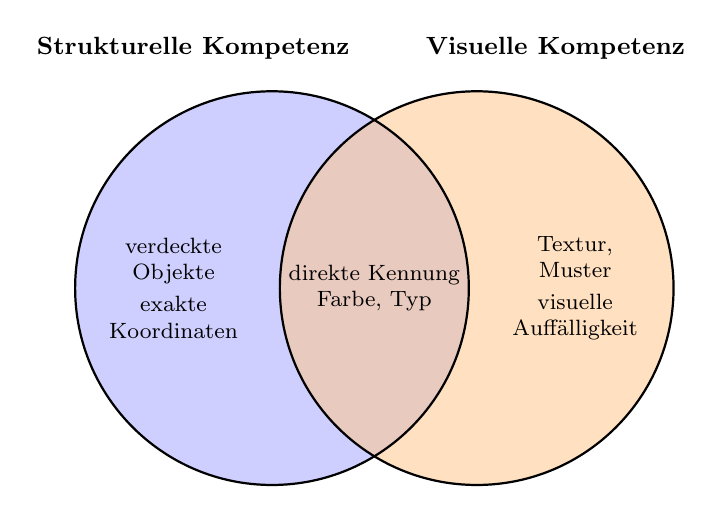
\begin{tikzpicture}[font=\small]
    \begin{scope}[fill opacity=0.55]
      \fill[blue!35]   (-1.3,0) circle (2.5);
      \fill[orange!45] ( 1.3,0) circle (2.5);
    \end{scope}
    \draw[thick] (-1.3,0) circle (2.5);
    \draw[thick] ( 1.3,0) circle (2.5);
    \node[font=\small\bfseries] at (-2.3,3.05) {Strukturelle Kompetenz};
    \node[font=\small\bfseries] at ( 2.3,3.05) {Visuelle Kompetenz};
    \node[align=center, font=\footnotesize] at (-2.55,0)
      {verdeckte\\Objekte\\[2pt]exakte\\Koordinaten};
    \node[align=center, font=\footnotesize] at (0,0)
      {direkte Kennung\\Farbe, Typ};
    \node[align=center, font=\footnotesize] at (2.55,0)
      {Textur,\\Muster\\[2pt]visuelle\\Auffälligkeit};
  \end{tikzpicture}
  \caption{Konzeptionelle Kompetenzverteilung der beiden Repräsentationen. Der Überlappungsbereich steht für Referenzen, die beide Schichten auflösen können, die Außenbereiche für die exklusive Kompetenz jeweils einer Schicht. Aus diesen exklusiven Bereichen ergibt sich der Nutzen des hybriden Ansatzes.}
  \label{fig:venn}
\end{figure}

% ============================================================
% KAPITEL 5 — IMPLEMENTIERUNG
% ============================================================

\chapter{Implementierung}
\label{ch:implementierung}

Dieses Kapitel beschreibt, wie das Konzept in ein lauffähiges System umgesetzt ist: den Aufbau im Überblick, die Anbindung der Szene, den Agenten mit seinen Werkzeugen, die fünf Repräsentationsvarianten und den VR-Demonstrator.


% ------------------------------------------------------------
\section{Systemüberblick}
\label{sec:impl-overview}

Das System verbindet einen natürlichsprachlichen Befehl mit einer sichtbaren Veränderung der 3D-Szene.
Es besteht aus drei lose gekoppelten Schichten, die über festgelegte Schnittstellen kommunizieren (Abbildung~\ref{fig:architektur}).

In der obersten Schicht deutet ein Agent den Befehl und wählt die nötige Manipulation.
Angetrieben wird er von einem lokal betriebenen Sprachmodell, für die visuelle Wahrnehmung greift er auf ein lokales visuelles Modell zurück.
Die mittlere Schicht ist ein Server nach dem Model Context Protocol (MCP)~\cite{mcp}.
Er stellt die Manipulationsoperationen als aufrufbare Werkzeuge bereit und übersetzt jeden Aufruf in eine Nachricht an die Umgebung; eine WebSocket-Verbindung transportiert diese Nachrichten und liefert Szenenzustand und gerenderte Bilder zurück.
Die unterste Schicht ist die Umgebung selbst, die die Szene hält, darstellt und die Manipulationen ausführt.
In der Evaluation läuft sie am Desktop, im Demonstrator auf der Meta Quest.
Weil die Schichten nur über diese Schnittstellen verbunden sind, lässt sich die Umgebung austauschen, ohne die übrigen Schichten zu verändern, und dieselbe Kette kann für die Messung und für den Demonstrator genutzt werden.

Ein Durchlauf beginnt mit dem Befehl an den Agenten.
Dieser fordert über die Werkzeuge zunächst den strukturellen Zustand oder eine gerenderte Ansicht an, entscheidet dann, welche Operation auszuführen ist, und ruft das passende Werkzeug auf.
Der MCP-Server leitet den Aufruf über die WebSocket-Verbindung an die Umgebung weiter, die die Manipulation ausführt.
Anschließend liest die Auswertung den neuen Szenenzustand aus und bestimmt daraus den Erfolg.

\begin{figure}[htbp]
  \centering
  \resizebox{\linewidth}{!}{%
  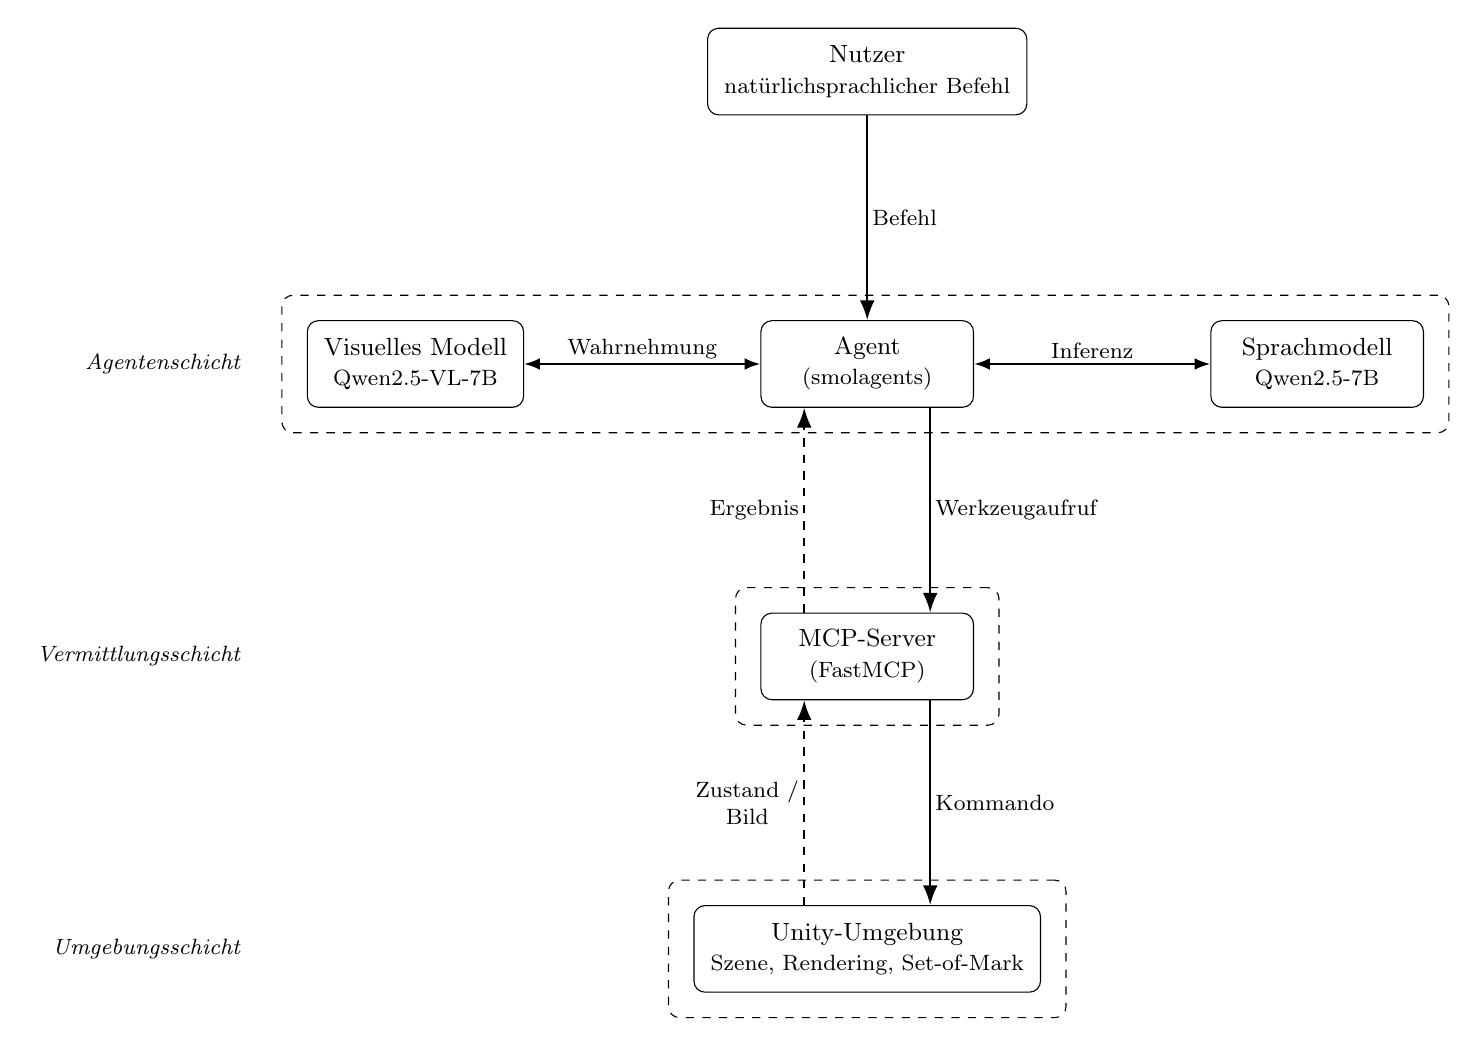
\begin{tikzpicture}[
      font=\small,
      box/.style={draw, rounded corners, align=center, inner sep=6pt,
                  minimum height=11mm, minimum width=27mm, fill=white},
      lbl/.style={font=\footnotesize, fill=white, inner sep=1.5pt},
      layer/.style={draw, dashed, rounded corners, inner sep=9pt},
      flow/.style={-{Latex[length=2.5mm]}, thick},
      back/.style={-{Latex[length=2.5mm]}, thick, dashed},
      exch/.style={{Latex[length=2mm]}-{Latex[length=2mm]}, thick},
      node distance=26mm and 30mm
    ]

    % --- Knoten ---
    \node[box] (user) {Nutzer\\{\footnotesize natürlichsprachlicher Befehl}};
    \node[box, below=of user] (agent) {Agent\\{\footnotesize (smolagents)}};
    \node[box, left=of agent]  (vlm) {Visuelles Modell\\{\footnotesize Qwen2.5-VL-7B}};
    \node[box, right=of agent] (llm) {Sprachmodell\\{\footnotesize Qwen2.5-7B}};
    \node[box, below=of agent] (mcp) {MCP-Server\\{\footnotesize (FastMCP)}};
    \node[box, below=of mcp]   (unity) {Unity-Umgebung\\{\footnotesize Szene, Rendering, Set-of-Mark}};

    % --- Nutzer -> Agent ---
    \draw[flow] (user) -- node[lbl, right]{Befehl} (agent);

    % --- Agent <-> Modelle ---
    \draw[exch] (agent) -- node[lbl, above]{Wahrnehmung} (vlm);
    \draw[exch] (agent) -- node[lbl, above]{Inferenz} (llm);

    % --- Agent <-> MCP ---
    \draw[flow] ([xshift=8mm]agent.south) -- node[lbl, right]{Werkzeugaufruf} ([xshift=8mm]mcp.north);
    \draw[back] ([xshift=-8mm]mcp.north)  -- node[lbl, left]{Ergebnis} ([xshift=-8mm]agent.south);

    % --- MCP <-> Unity ---
    \draw[flow] ([xshift=8mm]mcp.south)   -- node[lbl, right]{Kommando} ([xshift=8mm]unity.north);
    \draw[back] ([xshift=-8mm]unity.north)-- node[lbl, left, align=center]{Zustand /\\Bild} ([xshift=-8mm]mcp.south);

    % --- Schichten (Hintergrund) ---
    \begin{scope}[on background layer]
      \node[layer, fit=(vlm)(agent)(llm)] (L1) {};
      \node[layer, fit=(mcp)]   (L2) {};
      \node[layer, fit=(unity)] (L3) {};
    \end{scope}

    % --- Schicht-Beschriftungen ---
    \node[font=\footnotesize\itshape, anchor=east, xshift=-4mm] at (L1.west) {Agentenschicht};
    \node[font=\footnotesize\itshape, anchor=east, xshift=-4mm] at (L1.west |- L2) {Vermittlungsschicht};
    \node[font=\footnotesize\itshape, anchor=east, xshift=-4mm] at (L1.west |- L3) {Umgebungsschicht};

  \end{tikzpicture}%
  }
  \caption{Aufbau des Systems in drei Schichten und Nachrichtenfluss einer Manipulation. Durchgezogene Pfeile zeigen den Vorwärtsfluss, gestrichelte Pfeile den Rückkanal. Die Verbindung zwischen MCP-Server und Umgebung wird über WebSocket übertragen.}
  \label{fig:architektur}
\end{figure}


% ------------------------------------------------------------
\section{Szenenanbindung}
\label{sec:impl-scene}

Die Umgebung stellt die Szene in zwei Sichten bereit, einer strukturellen und einer visuellen.

Für die strukturelle Sicht führt die Umgebung intern ein Verzeichnis aller manipulierbaren Objekte und serialisiert es auf Anfrage als JSON.
Die Ausgabe enthält für jedes Objekt eine eindeutige Kennung, den Objekttyp, die Farbe, die Größe und die Position sowie zusätzlich die Pose der Kamera (Listing~\ref{lst:state}).
Die Kamerapose ist enthalten, damit sich auch Aufgaben lösen lassen, die sich auf den Betrachter beziehen.
Eigenschaften des Aussehens, die über die Grundfarbe hinausgehen, etwa eine Oberflächentextur, fehlen dagegen; deshalb sind rein perzeptuelle Referenzen über den strukturellen Zustand nicht auflösbar.

\begin{listing}[htbp]
\begin{minted}{json}
{
  "type": "state",
  "objects": [
    {"id": "obj_1", "type": "cube",   "color": "red",  "x": 0.0, "y": 0.0, "z": 0.0, "scale": 1.0},
    {"id": "obj_2", "type": "sphere", "color": "blue", "x": 2.0, "y": 0.0, "z": 0.0, "scale": 1.0}
  ],
  "camera": {
    "position": [0.0, 1.6, -6.0],
    "forward":  [0.0, 0.0, 1.0],
    "up":       [0.0, 1.0, 0.0]
  }
}
\end{minted}
\caption{Beispiel des strukturellen Szenenzustands als JSON-Ausgabe der Umgebung.}
\label{lst:state}
\end{listing}

Für die visuelle Sicht rendert die Umgebung die Szene aus der Kamera und übergibt das Bild.
Damit das visuelle Modell ein erkanntes Objekt auch für einen Werkzeugaufruf benennen kann, erhält jedes sichtbare Objekt nach dem Set-of-Mark-Prinzip~\cite{yang2023} eine gelbe, nummerierte Marke oberhalb seiner Bildposition.
Eine Zuordnungstabelle übersetzt die vom visuellen Modell genannten Nummern zurück in die Objektkennungen.
Beide Sichten verweisen damit auf dieselben Kennungen, sodass der Agent Objekte unabhängig von der Repräsentationsform einheitlich anspricht, wie es Abschnitt~\ref{sec:konz-fairness} verlangt.
Abbildung~\ref{fig:setofmark} zeigt dieselbe Szene ohne und mit Marken.

\begin{figure}[htbp]
  \centering
  \begin{minipage}{0.48\linewidth}
    \centering
    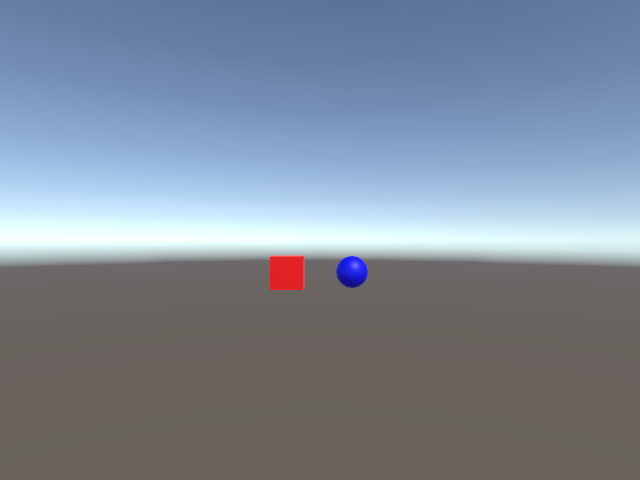
\includegraphics[width=\linewidth]{figures/scene}
  \end{minipage}\hfill
  \begin{minipage}{0.48\linewidth}
    \centering
    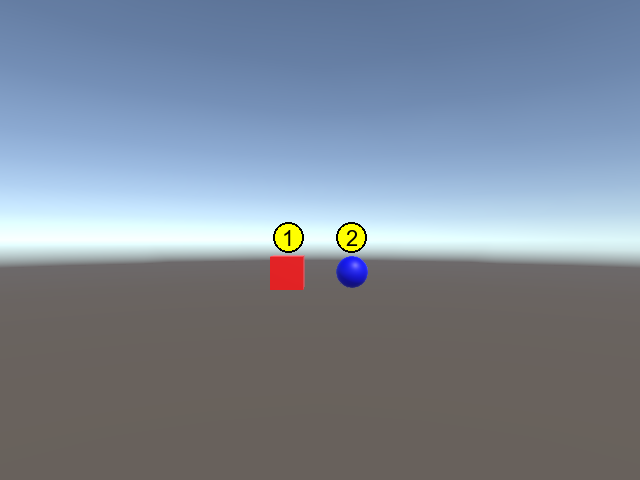
\includegraphics[width=\linewidth]{figures/scene_marked}
  \end{minipage}
  \caption{Die visuelle Repräsentation am Beispiel einer einfachen Szene. Links die gerenderte Ansicht, wie sie die Kamera liefert. Rechts dieselbe Ansicht nach dem Set-of-Mark-Verfahren, bei dem jedes sichtbare Objekt eine nummerierte Marke trägt, über die das visuelle Modell es benennen kann. Die Marken sind reine Bezeichner; ihre Farbe ist bedeutungslos und wird bei der Auswertung ignoriert.}
  \label{fig:setofmark}
\end{figure}

Eine Marke wird nur gesetzt, wenn das Objekt tatsächlich sichtbar ist.
Dazu prüft ein einzelner Sichtstrahl von der Kamera zum Objektmittelpunkt, ob ein anderes Objekt die Sichtlinie unterbricht; ist das der Fall, gilt das Objekt als verdeckt und bleibt unmarkiert.
Ein verdecktes Objekt fehlt dann in der visuellen Sicht vollständig, im strukturellen Zustand ist es aber weiterhin verzeichnet.
Auf dieser Asymmetrie beruhen die Testfälle, in denen ein Befehl auf ein im Bild unsichtbares Objekt verweist und die Abschnitt~\ref{sec:eval-taxonomy} als eigenen Referenztyp einführt.
Der Test ist binär und kennt keine Teilverdeckung.
Für die verwendeten Szenen, in denen ein Objekt entweder frei steht oder vollständig hinter einer großen Wand liegt, reicht das aus, für dichtere Szenen nicht.


% ------------------------------------------------------------
\section{Agent und Werkzeuge}
\label{sec:impl-agent}

Als Agent dient ein werkzeugaufrufender Agent aus dem Framework smolagents~\cite{smolagents}.
Angetrieben wird er von einem lokal betriebenen Sprachmodell, das über eine OpenAI-kompatible Schnittstelle angesprochen wird, die LM Studio auf dem Rechner bereitstellt.
In jedem Schritt der Agentenschleife entscheidet das Sprachmodell anhand des aktuellen Kontexts, welches Werkzeug mit welchen Argumenten aufgerufen wird, bis es die Aufgabe als abgeschlossen meldet.
Abbildung~\ref{fig:zyklus} zeigt diesen Ablauf von der Wahrnehmung bis zur Erfolgsbestimmung.
Da die Modelle nicht nachtrainiert werden, lässt sich ihr Verhalten nur über die Gestaltung des Kontexts steuern, und hier setzt die zweite Forschungsfrage an.

\begin{figure}[htbp]
  \centering
  \resizebox{\linewidth}{!}{%
  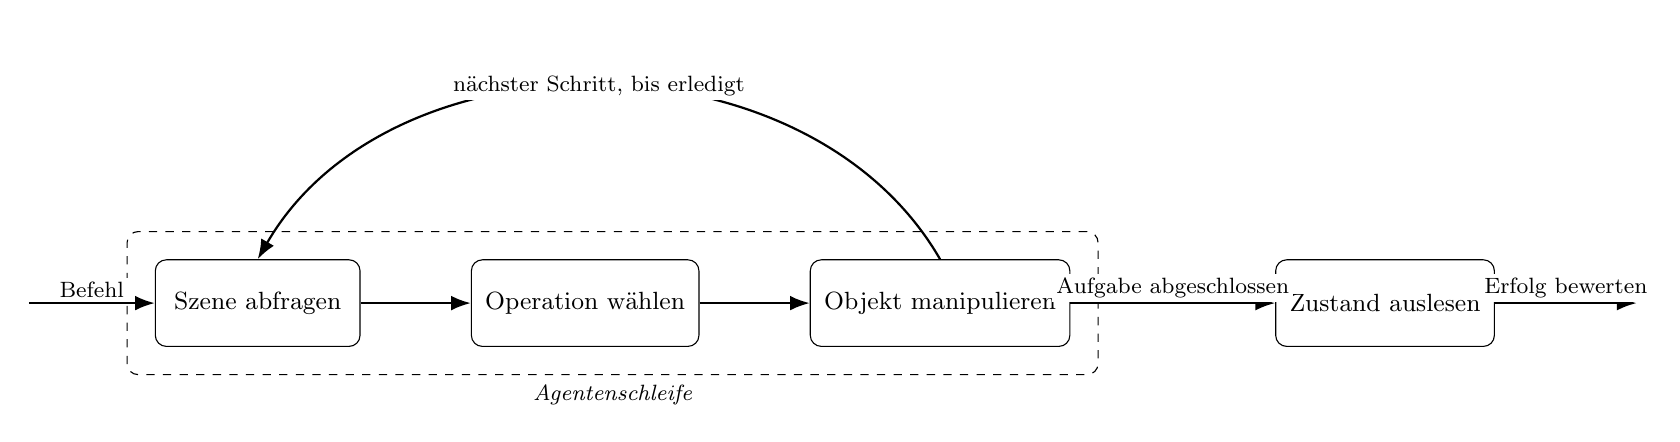
\begin{tikzpicture}[
      font=\small,
      box/.style={draw, rounded corners, align=center, inner sep=5pt,
                  minimum height=11mm, minimum width=26mm, fill=white},
      lbl/.style={font=\footnotesize, fill=white, inner sep=1.5pt},
      flow/.style={-{Latex[length=2.5mm]}, thick},
      node distance=14mm
    ]
    \node[box] (wahr) {Szene abfragen};
    \node[box, right=of wahr] (entsch) {Operation wählen};
    \node[box, right=of entsch] (aus) {Objekt manipulieren};
    \node[box, right=26mm of aus] (pruef) {Zustand auslesen};

    % Eintritt
    \draw[flow] ([xshift=-16mm]wahr.west) -- node[lbl, above]{Befehl} (wahr.west);
    % lineare Kette
    \draw[flow] (wahr) -- (entsch);
    \draw[flow] (entsch) -- (aus);
    \draw[flow] (aus) -- node[lbl, above]{Aufgabe abgeschlossen} (pruef);
    % Austritt
    \draw[flow] (pruef.east) -- node[lbl, above]{Erfolg bewerten} ([xshift=18mm]pruef.east);
    % Schleife oberhalb der drei Agentenschritte
    \draw[flow] (aus.north) to[out=120, in=60] node[lbl]{nächster Schritt, bis erledigt} (wahr.north);

    % Agentenschleife als gestrichelte Gruppe
    \begin{scope}[on background layer]
      \node[draw, dashed, rounded corners, inner sep=10pt, fit=(wahr)(entsch)(aus)] (loopbox) {};
    \end{scope}
    \node[font=\footnotesize\itshape, anchor=north] at (loopbox.south) {Agentenschleife};
  \end{tikzpicture}%
  }
  \caption{Ablauf einer einzelnen Manipulation. In der Agentenschleife fragt der Agent die Szene über ein Wahrnehmungswerkzeug ab, das Sprachmodell wählt die passende Operation, und das gewählte Werkzeug manipuliert das Objekt. Diese Schritte wiederholen sich, bis der Agent die Aufgabe abschließt. Danach liest die Auswertung den tatsächlichen Szenenzustand aus und bewertet daraus den Erfolg, unabhängig von der Selbstauskunft des Agenten.}
  \label{fig:zyklus}
\end{figure}

Die Operationen selbst stellt der MCP-Server als Werkzeuge bereit.
Die manipulierenden Werkzeuge erzeugen, verschieben und entfernen Objekte oder setzen die Szene zurück, die wahrnehmenden liefern den strukturellen Zustand oder eine gerenderte Ansicht.
Jedes Werkzeug trägt eine kurze Beschreibung als Dokumentationskommentar, und diese Beschreibung ist es, die der Agent bei der Wahl des nächsten Aufrufs sieht.
Listing~\ref{lst:tool} zeigt den Aufbau am Beispiel des Verschiebens.

\begin{listing}[htbp]
\begin{minted}{python}
@mcp.tool()
def move_object(object_id: str, x: float, y: float, z: float) -> str:
    """Move an existing object (id from get_scene_state) to a new position."""
    global _last_op
    key = ("move", object_id, x, y, z)
    if key == _last_op:                 # Schutz gegen doppelte Ausfuehrung
        return f"Skipped: identical move already applied to {object_id}."
    _last_op = key
    send_to_unity({"action": "move", "id": object_id, "x": x, "y": y, "z": z})
    return f"Done: {object_id} moved to ({x}, {y}, {z})."
\end{minted}
\caption{Beispiel einer Werkzeugdefinition (gekürzt). Der Dokumentationskommentar dient dem Agenten als Beschreibung des Werkzeugs.}
\label{lst:tool}
\end{listing}

\subsection*{Schutz gegen doppelte Ausführung}

Der Erfolg einer Manipulation wird aus dem tatsächlichen Folgezustand der Szene bestimmt (Abschnitt~\ref{sec:eval-metrics}), und damit hängt ein Detail der Werkzeuge zusammen.
Das lokale Modell bündelte gelegentlich einen Manipulations- und einen Abschlussaufruf so, dass dieselbe Manipulation zweimal ausgeführt wurde.
Um dieses Verhalten des Frameworks zu neutralisieren, vergleicht jedes manipulierende Werkzeug den aktuellen Aufruf mit dem unmittelbar vorangegangenen und überspringt eine identische Wiederholung (Abfrage von \texttt{\_last\_op} in Listing~\ref{lst:tool}).

Der Schutz ist grob, denn er kann nicht unterscheiden, ob eine identische Wiederholung ein Artefakt des Frameworks ist oder vom Befehl verlangt wird.
Ein Befehl, der dieselbe Operation absichtlich zweimal fordert, würde ebenfalls blockiert.
In den ausgewerteten Szenarien kommt das nicht vor, da kein Soll-Ergebnis zwei identische Aufrufe erfordert; bei Mehrschritt-Befehlen ließe es sich aber nicht ausschließen.


% ------------------------------------------------------------
\section{Repräsentationsvarianten}
\label{sec:impl-variants}

Alle fünf Varianten teilen denselben Agenten und dieselbe Grundinstruktion.
Diese verlangt, vor jeder Manipulation zuerst die Szene wahrzunehmen, keine Kennung zu erfinden, die Aufgabe mit einem einzigen Manipulationsaufruf zu lösen und danach abzuschließen.
Die letzte Vorgabe ist eine Vereinfachung, die nicht zu allen Szenarien passt: Zwei Szenarien betreffen ihrem Soll-Ergebnis nach mehrere Objekte, was Abschnitt~\ref{sec:eval-validity} diskutiert.

Die Varianten unterscheiden sich allein im Wahrnehmungswerkzeug, das dem Agenten zur Verfügung steht.
Gesteuert wird die Gewichtung der beiden Schichten über zwei Stellen: den Dokumentationskommentar des Werkzeugs, den der Agent bei der Wahl des nächsten Aufrufs liest, und den zurückgegebenen Text, der die beiden Schichten benennt und ordnet.

\subsection*{Strukturelle und visuelle Variante}

Die strukturelle Variante hat nur Zugriff auf den strukturellen Zustand, also auf das JSON mit Kennungen, Typen, Farben, Größen und Positionen, aber auf kein Bild.
Die visuelle Variante erhält nur eine Beschreibung der gerenderten und markierten Ansicht und kennt die Objekte damit nur über ihre Marken und sichtbaren Eigenschaften, ohne exakte Koordinaten.
Diese Beschreibung erzeugt das visuelle Modell aus dem Bild; das Bild selbst gelangt nie in den Kontext des Agenten (Abschnitt~\ref{sec:grundlagen-modelle}).
Auch die hybriden Varianten kombinieren daher zwei Textquellen, den JSON-Zustand und die erzeugte Beschreibung.

Was die Beschreibung enthält, legt der Prompt fest, mit dem das visuelle Modell das Bild beschreibt (Listing~\ref{lst:vlmprompt}).
Er wird in allen Varianten mit visueller Schicht unverändert verwendet und ist damit ein fester, nicht variierter Teil des Aufbaus.
Der Prompt weist das Modell ausdrücklich an, die Farbe der Marke zu ignorieren und die tatsächliche Objektfarbe zu berichten; diese Anweisung geht auf einen in Abschnitt~\ref{sec:eval-validity} beschriebenen Störfaktor zurück.

\begin{listing}[htbp]
\begin{minted}[breaklines]{python}
"Each object has a yellow numbered badge floating above it. Badges are
labels ONLY - ignore badge color; report the actual object color. For
each numbered object give number, shape (cube/sphere/cylinder), color,
qualitative position, and a surface texture descriptor (e.g. 'striped'
or 'solid'). Answer ONLY as a JSON list with keys: number, shape,
color, position, texture."
\end{minted}
\caption{Prompt, mit dem das visuelle Modell die gerenderte und markierte Ansicht beschreibt. Er wird zusammen mit dem Bild übergeben und ist in allen Varianten mit visueller Schicht identisch.}
\label{lst:vlmprompt}
\end{listing}

Zwei Eigenschaften des Prompts wirken sich auf die Ergebnisse aus.
Er verlangt je Objekt fünf Angaben, nämlich Nummer, Form, Farbe, qualitative Lage und einen Texturdeskriptor, aber keine Größe; was die visuelle Schicht über Größen berichtet, steht allenfalls zufällig in der Lagebeschreibung.
Außerdem nennt er als Beispiel für einen Texturdeskriptor \enquote{striped}, ein Wort, das auch in den Befehlen der perzeptuellen Szenarien vorkommt.
Da alle Varianten mit visueller Schicht denselben Prompt nutzen, verschafft das keiner einzelnen Variante einen Vorteil, schränkt aber die Aussagekraft der Kategorie~D ein.
Auf beide Punkte kommen die Abschnitte~\ref{sec:eval-rq1} und~\ref{sec:eval-validity} zurück.

\subsection*{Hybride Varianten}

Die naive hybride Variante stellt beide Schichten nebeneinander.
Sie gibt zuerst den strukturellen Zustand und danach die visuelle Beschreibung aus und deutet nur grob an, wofür welche Schicht gedacht ist; eine verbindliche Zuständigkeitsregel fehlt (Listing~\ref{lst:hybrid}).

\begin{listing}[htbp]
\begin{minted}{python}
@tool
def get_scene_hybrid() -> str:
    """Perceive the scene using BOTH exact structural data (ids, positions,
    colors, sizes, camera) and a visual description. Use exact data for
    geometry, visual data for semantics."""
\end{minted}
\caption{Wahrnehmungswerkzeug der naiven hybriden Variante.}
\label{lst:hybrid}
\end{listing}

Die priorisierende Variante, im Code \texttt{guided}, setzt die erste Strategie aus Abschnitt~\ref{sec:konz-fusion} um.
Sie stellt die visuelle Beschreibung voran und erklärt sie für das Aussehen als maßgeblich, während die strukturelle Schicht ausdrücklich als rein geometrisch und frei von Aussehens-Information gekennzeichnet wird (Listing~\ref{lst:guided}).
Das Gewicht verschiebt sich damit zugunsten der visuellen Beschreibung.

\begin{listing}[htbp]
\begin{minted}{python}
@tool
def get_scene_hybrid_guided() -> str:
    """Perceive the scene using a visual description AND exact structural
    data. The visual description is authoritative for how objects LOOK
    (texture, pattern, whether something stands out). The structural data
    contains ONLY geometry (positions, sizes, base colors) and does NOT
    encode any visual surface property."""
\end{minted}
\caption{Wahrnehmungswerkzeug der priorisierenden Variante.}
\label{lst:guided}
\end{listing}

Die kompetenzgetrennte Variante, im Code \texttt{surgical}, setzt die zweite Strategie um.
Wie die naive Variante gibt sie den strukturellen Zustand zuerst aus, weist den Schichten aber ausdrücklich getrennte Aufgaben zu (Listing~\ref{lst:surgical}).
Die visuelle Beschreibung dient nur dazu, das gemeinte Objekt zu bestimmen, wenn die Referenz vom Aussehen abhängt; alles Numerische, also Koordinaten, Größen, Abstände und Kamerageometrie, kommt aus der strukturellen Schicht.
Von der priorisierenden Variante unterscheidet sie sich also vor allem durch diese enge, gegenseitig ausschließende Zuweisung und erst in zweiter Linie durch die Reihenfolge.

\begin{listing}[htbp]
\begin{minted}{python}
@tool
def get_scene_hybrid_surgical() -> str:
    """Perceive the scene using a visual description AND exact structural
    data, with a clear division of labor. Use the VISUAL description ONLY
    to identify WHICH object is meant when the reference depends on
    appearance (texture, pattern, 'striped', 'stands out', 'most salient').
    Use the STRUCTURAL data for EVERYTHING numerical: all coordinates,
    positions, sizes, distances, camera geometry, and to compute where to
    move things. Every object id appears in both - match them by id.
    Never take coordinates from the visual description; never resolve an
    appearance-based reference from the structural data alone."""
\end{minted}
\caption{Wahrnehmungswerkzeug der kompetenzgetrennten Variante.}
\label{lst:surgical}
\end{listing}

Die kompetenzgetrennte Variante wurde nicht vorab entworfen, sondern iterativ entwickelt.
Ausgangspunkt war die Beobachtung, dass die naive Kombination in einem Teil der perzeptuellen Szenarien den visuellen Zugriff verliert und die Priorisierung das zwar behebt, dafür aber metrische Aufgaben schwächt.
Daraus entstand die Idee, den Schichten getrennte Rollen zu geben, statt eine von ihnen zu bevorzugen.
Die Formulierung wurde in mehreren Schritten geschärft, jeweils in Kenntnis der Ergebnisse der vorigen Läufe und auf demselben Szenarioset, auf dem die Variante anschließend berichtet wird.
Die Spuren davon sind in Listing~\ref{lst:surgical} zu sehen: \enquote{striped} und \enquote{most salient} kommen wörtlich in den Befehlen der Szenarien D1 und D2 vor.
Was das für die Reichweite des Befundes bedeutet, diskutiert Abschnitt~\ref{sec:eval-validity}.

Tabelle~\ref{tab:variants} fasst die Varianten zusammen.
Sie nennt auch die Kurzbezeichnungen aus dem Code, die in den Ergebnistabellen als Spaltenköpfe erscheinen; im Fließtext werden die deutschen Bezeichnungen verwendet.
An der Spalte \enquote{Im Kontext} ist abzulesen, dass sich die priorisierende Variante von den beiden anderen hybriden Varianten auch in der Reihenfolge der Schichten unterscheidet, Instruktion und Reihenfolge also nicht getrennt variiert sind.

\begin{table}[htbp]
  \centering
  \caption{Die fünf Repräsentationsvarianten im Vergleich, mit den in den Ergebnistabellen verwendeten Kurzbezeichnungen.}
  \label{tab:variants}
  \small
  \setlength{\tabcolsep}{5pt}
  \renewcommand{\arraystretch}{1.3}
  \begin{tabular}{@{}p{3.0cm} l p{3.3cm} p{4.6cm}@{}}
    \toprule
    Variante & Kurzform & Im Kontext & Regel zur Gewichtung \\
    \midrule
    strukturell & \texttt{json} & nur struktureller Zustand & entfällt, keine visuelle Schicht \\
    visuell & \texttt{vlm} & nur visuelle Beschreibung & entfällt, keine strukturelle Schicht \\
    naiv hybrid & \texttt{hybrid} & Struktur, dann Beschreibung & grobe Zuordnung ohne verbindliche Regel \\
    priorisierend & \texttt{guided} & Beschreibung, dann Struktur & Beschreibung maßgeblich fürs Aussehen, Struktur nur Geometrie \\
    kompetenzgetrennt & \texttt{surgical} & Struktur, dann Beschreibung & Beschreibung nur zur Objektwahl, Struktur für alles Numerische \\
    \bottomrule
  \end{tabular}
\end{table}


% ------------------------------------------------------------
\section{VR-Demonstrator}
\label{sec:impl-demonstrator}

Die Evaluation lief am Desktop unter kontrollierten Bedingungen.
Um zu zeigen, dass der Ansatz auch in der eigentlichen Zielumgebung funktioniert, überführt ein Demonstrator die gesamte Kette in die immersive Umgebung.
Er nutzt die kompetenzgetrennte Variante, die sich in Kapitel~\ref{ch:evaluation} auf dem untersuchten Szenarioset als die zuverlässigste erweist.
Der Demonstrator ist lokal im Sinne von Abschnitt~\ref{sec:ein-motivation}: Alle Modelle sind selbst gehostet, kein Cloud-Dienst ist beteiligt, und keine Szenen- oder Sprachdaten verlassen das Institutsnetz.
Gerechnet wird aber nicht auf der Brille, sondern auf dem Arbeitsplatzrechner, den die Brille über die unten beschriebene Netzwerkkette erreicht.

\subsection*{Sprachsteuerung}

Der Nutzer spricht einen Befehl, und ein selbst gehostetes Whisper-Modell in der Größe \texttt{small} wandelt die Aufnahme in Text um.
Es läuft auf dem lokalen Rechner auf der CPU, nimmt mit 16\,kHz auf und ist passend zur Sprache der Befehle auf englische Eingaben festgelegt.
Der erkannte Text landet in derselben Kommando-Warteschlange, die auch in der Evaluation den Agenten antreibt; ein gesprochener Befehl durchläuft also dieselbe Kette wie ein Befehl im Experiment, nur mit vorgeschalteter Spracherkennung (Abbildung~\ref{fig:voicechain}).

Über dieselbe Verbindung treten dabei zwei Arten von Clients auf.
Die Brille ist der Renderer, der die Manipulationen ausführt und die Szene darstellt, die Sprachsteuerung der Commander, der nur Befehle einspeist.
Eine Anmeldenachricht unterscheidet die beiden Rollen, damit die Befehlsquelle die Verbindung der Brille nicht verdrängt.
Sobald ein Befehl in der Warteschlange liegt, arbeitet ein Worker den Agentenlauf ab und meldet der Brille Beginn und Abschluss der Verarbeitung, sodass der Nutzer sieht, dass sein Befehl gerade bearbeitet wird.

\begin{figure}[htbp]
  \centering
  \resizebox{0.9\linewidth}{!}{%
  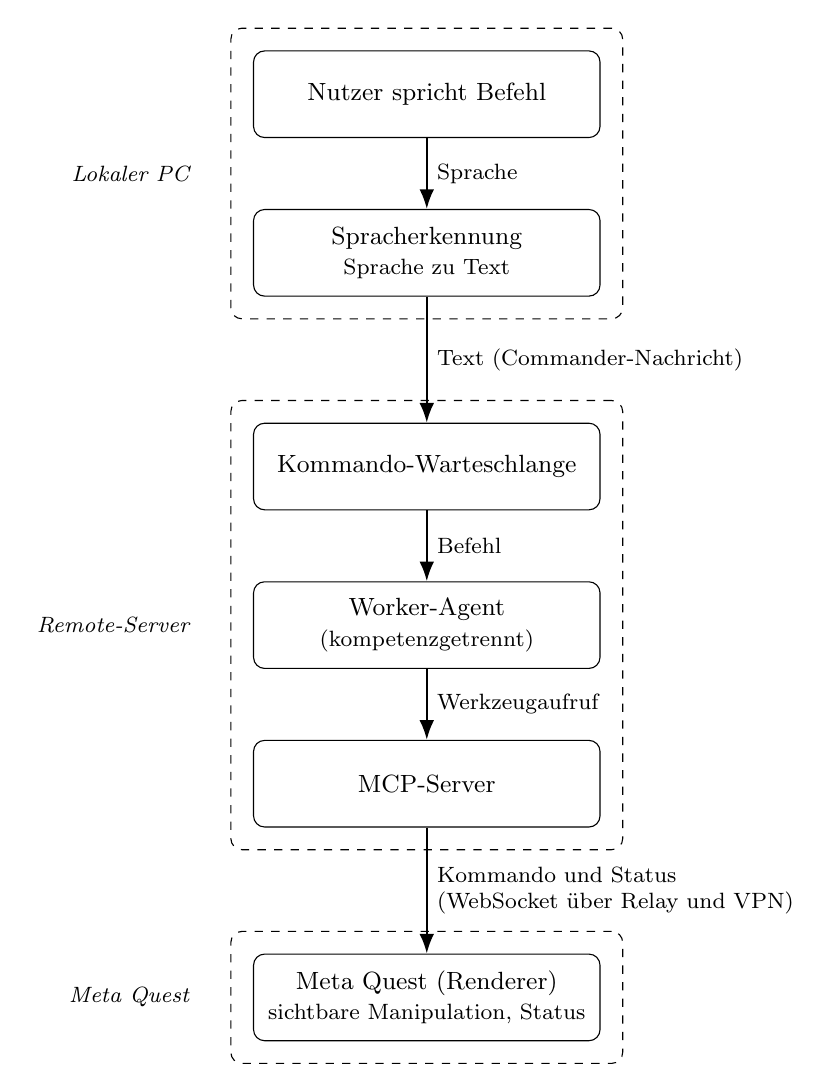
\begin{tikzpicture}[
      font=\small,
      box/.style={draw, rounded corners, align=center, inner sep=5pt,
                  minimum height=11mm, minimum width=44mm, fill=white},
      band/.style={draw, dashed, rounded corners, inner sep=8pt},
      flow/.style={-{Latex[length=2.5mm]}, thick},
      node distance=9mm
    ]
    \node[box] (user) {Nutzer spricht Befehl};
    \node[box, below=of user] (whisper) {Spracherkennung\\{\footnotesize Sprache zu Text}};
    \node[box, below=16mm of whisper] (queue) {Kommando-Warteschlange};
    \node[box, below=of queue] (agent) {Worker-Agent\\{\footnotesize (kompetenzgetrennt)}};
    \node[box, below=of agent] (mcp) {MCP-Server};
    \node[box, below=16mm of mcp] (quest) {Meta Quest (Renderer)\\{\footnotesize sichtbare Manipulation, Status}};

    \draw[flow] (user) -- node[right, font=\footnotesize]{Sprache} (whisper);
    \draw[flow] (whisper) -- node[right, font=\footnotesize]{Text (Commander-Nachricht)} (queue);
    \draw[flow] (queue) -- node[right, font=\footnotesize]{Befehl} (agent);
    \draw[flow] (agent) -- node[right, font=\footnotesize]{Werkzeugaufruf} (mcp);
    \draw[flow] (mcp) -- node[right, font=\footnotesize, align=left]{Kommando und Status\\(WebSocket über Relay und VPN)} (quest);

    \begin{scope}[on background layer]
      \node[band, fit=(user)(whisper)] (b1) {};
      \node[band, fit=(queue)(agent)(mcp)] (b2) {};
      \node[band, fit=(quest)] (b3) {};
    \end{scope}
    \node[font=\footnotesize\itshape, anchor=east, xshift=-4mm] at (b2.west |- b1) {Lokaler PC};
    \node[font=\footnotesize\itshape, anchor=east, xshift=-4mm] at (b2.west) {Remote-Server};
    \node[font=\footnotesize\itshape, anchor=east, xshift=-4mm] at (b2.west |- b3) {Meta Quest};

  \end{tikzpicture}%
  }
  \caption{Ablauf eines gesprochenen Befehls im Demonstrator. Der lokale Rechner erkennt die Sprache und leitet den Text als Commander-Nachricht weiter, der entfernte Rechner arbeitet den Agentenlauf ab, und die Brille führt die Manipulation aus und zeigt den Verarbeitungsstatus an.}
  \label{fig:voicechain}
\end{figure}

\subsection*{Wahrnehmung und Netzwerk}

Für die visuelle Wahrnehmung braucht das visuelle Modell ein flaches, gerendertes Bild.
Die Hauptkamera der Brille rendert jedoch stereoskopisch für beide Augen und liefert kein brauchbares Einzelbild.
Deshalb gibt es eine eigene Aufnahmekamera, die der Kopfpose folgt, aber einfach statt stereoskopisch rendert.

Die Modelle laufen aus Ressourcengründen auf dem Arbeitsplatzrechner im Institutsnetz, den die Brille nicht direkt erreicht.
Sie verbindet sich deshalb mit einem Vermittler auf einem Rechner im selben Funknetz, der die Nachrichten über ein virtuelles privates Netz an den Arbeitsplatzrechner weiterleitet.
Ein mobiler Zugangspunkt umgeht dabei die Isolation gemeinsam genutzter Netze, die eine direkte Verbindung sonst unterbindet.
Diese Kette ist reine Demonstrationsinfrastruktur und nicht Gegenstand der Untersuchung.

\subsection*{Ausbaustufen und Aufzeichnung}

Zuerst entstand eine Fassung mit einem Bedienmenü in der Szene, das vordefinierte Befehle bereitstellt und bereits dieselbe Kommando-Warteschlange nutzt; die Sprachsteuerung kam später hinzu.
Von dieser frühen Menüfassung gibt es eine Videoaufzeichnung aus der Sicht der Brille, die als Begleitmaterial beiliegt (Anhang~\ref{anh:video}) und aus der das Standbild in Abbildung~\ref{fig:demo} stammt.
Die Szene enthält einen roten Würfel links, einen gestreiften Würfel in der Mitte und eine blaue Kugel rechts; der gestreifte Würfel wird im Standbild von der Menütafel weitgehend verdeckt.
Im Video werden die vordefinierten Befehle nacheinander ausgelöst, und die Manipulationen sind jeweils unmittelbar zu sehen: Der gestreifte Würfel hebt sich an, die blaue Kugel wandert nach links neben den roten Würfel, und zuletzt wird der gestreifte Würfel entfernt.

Die Aufzeichnung belegt damit die Kette von der Befehlsauswahl über Agent und MCP-Server bis zur sichtbaren Manipulation in der Brille.
Die Spracheingabe ist umgesetzt und lauffähig, aber nicht aufgezeichnet und damit nicht per Video belegt.

\begin{figure}[htbp]
  \centering
  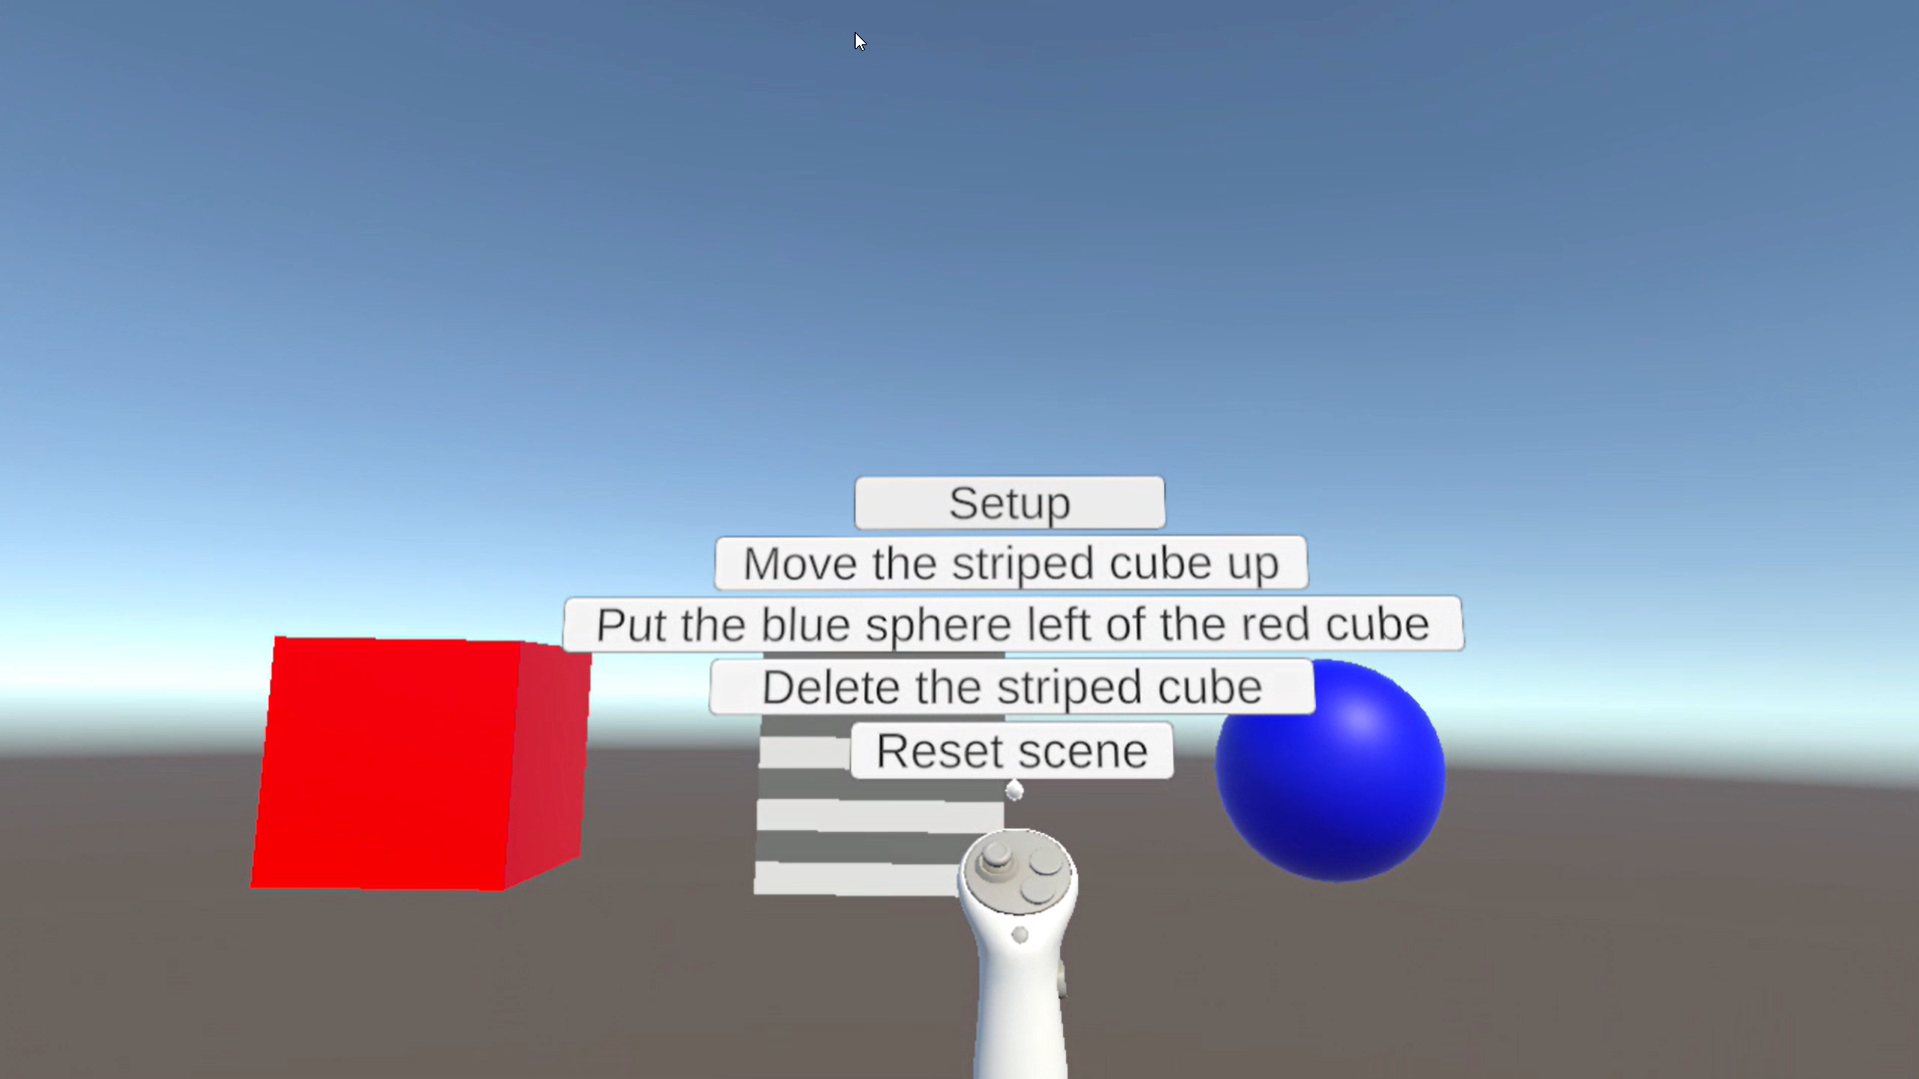
\includegraphics[width=0.7\linewidth]{figures/demo_still}
  \caption{Frühe Ausbaustufe des Demonstrators mit Bedienmenü. Links der rote Würfel, rechts die blaue Kugel; der gestreifte Würfel in der Mitte wird von der Menütafel weitgehend verdeckt, nur sein unterer Teil ist sichtbar. Das Standbild stammt aus der Aufzeichnung in Anhang~\ref{anh:video}, in der unter anderem \enquote{move the striped cube up}, \enquote{put the blue sphere left of the red cube} und \enquote{delete the striped cube} über das Menü ausgelöst werden.}
  \label{fig:demo}
\end{figure}

% ============================================================
% KAPITEL 6 — EVALUATION
% ============================================================

\chapter{Evaluation}
\label{ch:evaluation}

Dieses Kapitel vergleicht die Repräsentationsformen entlang einer nach Referenztypen aufgeschlüsselten Taxonomie und bestimmt, welche Form welche Art von Referenz trägt (RQ1).
Anschließend prüft es, ob sich die hybride Repräsentation allein über ihre Instruktion so gestalten lässt, dass sie die Stärken beider Schichten vereint (RQ2).
Zum Schluss werden Validität und Grenzen der Ergebnisse diskutiert.


% ------------------------------------------------------------
\section{Evaluationsdesign}
\label{sec:eval-design}

Verglichen werden die fünf Varianten aus Abschnitt~\ref{sec:impl-variants}.
Sie nutzen dieselben Szenen, Befehle und Manipulationswerkzeuge und unterscheiden sich allein darin, in welcher Form die Szene dem Agenten bereitgestellt wird.
Da alle Varianten Objekte über dasselbe Kennungssystem ansprechen (Abschnitt~\ref{sec:konz-fairness}), gehen gemessene Unterschiede nicht auf einen ungleichen Werkzeugzugriff zurück.
Für die Deutung ist dabei im Blick zu behalten, dass das entscheidende Sprachmodell in keiner Variante ein Bild erhält, sondern im visuellen Fall eine Beschreibung des Bildes (Abschnitt~\ref{sec:grundlagen-modelle}).
Streng genommen werden also eine exakte Datenstruktur und eine unscharfe sprachliche Beschreibung derselben Szene verglichen.

Ob eine Manipulation gelungen ist, wird aus dem tatsächlichen Zustand der Szene nach der Ausführung bestimmt, den die Auswertung mit der Soll-Vorgabe des Szenarios vergleicht (Abschnitt~\ref{sec:eval-metrics}).
Die Selbstauskunft des Agenten bleibt unberücksichtigt, weil das lokale Modell wiederholt Erfolge meldete, die der Folgezustand nicht bestätigte (Abschnitt~\ref{sec:eval-validity}).

Jede Kombination aus Szenario und Variante wird zehnmal ausgeführt und der gesamte Durchlauf dreimal wiederholt, sodass jede Zelle auf 30 Läufen beruht.
Berichtet wird der Mittelwert über die drei Durchläufe mit der Spanne von Minimum und Maximum, an der sich ablesen lässt, wie stark eine Zelle zwischen den Durchläufen schwankt.
Für die zentralen Vergleiche werden die 30 Läufe einer Zelle zusätzlich zusammengefasst und inferenzstatistisch ausgewertet.

Ausgewertet werden dreizehn Szenarien in fünf Kategorien.
Die Kategorien A, B und C umfassen je drei Szenarien, D und E nur je zwei, obwohl gerade diese beiden die inhaltlich zentralen Befunde tragen.
Die Szenen bestehen aus einfachen geometrischen Grundkörpern und sind so aufgebaut, dass jedes Szenario eine bestimmte Repräsentationskompetenz isoliert.
Gemessen wird am Desktop, weil sich die Szenen dort exakt kontrollieren und beliebig oft identisch wiederholen lassen; die immersive Umgebung ist nur Zielumgebung des Demonstrators.
Als Sprachmodell dient Qwen2.5-7B, als visuelles Modell Qwen2.5-VL-7B, beide selbst gehostet und gemeinsam auf einer NVIDIA RTX A5000 mit 24 Gigabyte Grafikspeicher.
Tabelle~\ref{tab:config} führt die vollständige Konfiguration auf, die nach NFA3 für eine Wiederholung der Messung nötig ist.

\begin{table}[htbp]
  \centering
  \caption{Konfiguration der Messung, beschränkt auf die Angaben, die den
           Ausgang der Läufe beeinflussen. Zusammen mit dem verlinkten Code
           genügen sie, um die Messung zu wiederholen.}
  \label{tab:config}
  \small
  \setlength{\tabcolsep}{5pt}
  \renewcommand{\arraystretch}{1.3}
  \begin{tabular}{@{}p{3.4cm} p{9.6cm}@{}}
    \toprule
    Größe & Wert \\
    \midrule
    Sprachmodell      & \texttt{qwen2.5-7b-instruct}, GGUF Q4\_K\_M, 4096 Token Kontext \\
    Visuelles Modell  & \texttt{qwen/qwen2.5-vl-7b}, GGUF Q4\_K\_M, 4096 Token Kontext \\
    Hardware, Laufzeit & NVIDIA RTX A5000 mit 24\,GB, LM Studio (CLI-Commit \texttt{efce996}), beide Modelle gleichzeitig geladen \\
    Agent             & smolagents 1.26.0 (\texttt{ToolCallingAgent}) unter Python 3.13, \texttt{max\_steps} = 6 \\
    Dekodierung       & Sprachmodell: Temperatur 0{,}8 (Voreinstellung der Laufzeitumgebung, im Client nicht überschrieben). Visuelles Modell: Temperatur 0{,}1 (im Client ausdrücklich gesetzt). Kein fester Seed \\
    Messumfang        & 13 Szenarien $\times$ 5 Varianten, je 10 Läufe in 3 Durchläufen, also 30 Läufe pro Zelle \\
    Code und Rohdaten & \url{https://git.informatik.fh-nuernberg.de/jobboerse/forschung/bachelorarbeiten/bachelorarbeit-sandro-jaeger} \\
    \bottomrule
  \end{tabular}
\end{table}

Beide Modelle liegen in derselben Quantisierungsstufe vor.
Eine unterschiedlich starke Quantisierung hätte die beiden Schichten ungleich beeinträchtigt und damit neben der Repräsentationsform eine weitere Störgröße eingeführt.
Mit 4{,}68\,GB und 6{,}04\,GB belegen die Gewichte zusammen rund 10{,}7\,GB, sodass auf der Karte Platz für den Schlüssel-Wert-Zwischenspeicher beider Modelle bleibt; erst dadurch ist der gleichzeitige Betrieb nach NFA2 möglich.

Knapp bemessen ist dagegen die Kontextlänge von 4096 Token, und sie trifft die Varianten ungleich.
Zusätzlich zu Grundinstruktion, Werkzeugbeschreibungen und bisherigem Verlauf der Agentenschleife trägt die strukturelle Variante nur den JSON-Zustand im Kontext, die visuelle nur die Beschreibung, die hybriden Varianten aber beides.
Für mehrere aufeinanderfolgende Schritte bleibt ihnen deshalb systematisch weniger Platz.
Ob sich das in den Messungen auswirkte, etwa durch abgeschnittenen Kontext in längeren Läufen, wurde nicht überwacht und lässt sich nachträglich nicht mehr feststellen.

Unterschiedlich ist auch die Dekodierung der beiden Modelle.
Das Sprachmodell, das die Entscheidung trifft, lief mit einer Temperatur von 0{,}8, einer Einstellung, die den Antwortraum spürbar öffnet.
Die zehn Läufe einer Zelle sind damit weitgehend unabhängige Ziehungen aus einer breiten Verteilung und keine Wiederholungen derselben Antwort.
Eine Zelle, die bei 0 von 30 oder bei 30 von 30 liegt, kommt also nicht dadurch zustande, dass das Modell ohnehin immer dasselbe antwortet, sondern trotz des Spielraums in der Dekodierung.
Die vielen Zellen ohne Streuung sind unter dieser Bedingung ein Befund und kein Artefakt einer zu niedrigen Temperatur: Der jeweilige Effekt wirkt stärker als das Rauschen.

Das visuelle Modell lief dagegen mit einer Temperatur von 0{,}1 und damit nahezu deterministisch, sodass die Beschreibung einer gegebenen Szene über die Läufe hinweg weitgehend gleich ausfällt.
Das ist gewollt, denn die Wahrnehmungsstufe ist Eingabe und nicht Untersuchungsgegenstand, und eine stark schwankende Beschreibung hätte eine zusätzliche Störgröße zwischen Repräsentationsform und Ergebnis geschoben.
Die Streuung einer Zelle geht damit fast vollständig auf das Sprachmodell zurück, also auf die Stufe, die verglichen wird.
Eine Restabhängigkeit zwischen den Läufen bleibt, weil alle Läufe einer Zelle dieselbe, nahezu unveränderliche Szenenbeschreibung nutzen; sie betrifft aber die Eingabe und nicht die gemessene Entscheidung.


% ------------------------------------------------------------
\section{Referenztyp-Taxonomie}
\label{sec:eval-taxonomy}

Welche Repräsentation eine Aufgabe trägt, hängt davon ab, worauf sich der Befehl bezieht.
Ein Verweis auf die Farbe eines Objekts stellt andere Anforderungen als ein Verweis auf seine Lage oder auf ein Objekt, das im Bild gar nicht zu sehen ist.
Eine pauschale Antwort auf die Frage nach der besten Repräsentation gibt es deshalb nicht.
Die Evaluation zerlegt die natürlichsprachliche Referenz stattdessen in fünf Typen und prüft für jeden einzeln, welche Repräsentation ihn auflösen kann.
Tabelle~\ref{tab:taxonomy} zeigt, in welcher Schicht die dafür nötige Information jeweils verfügbar ist.

Kategorie A ist die Kontrollbedingung.
Der Befehl benennt das Zielobjekt direkt über seine Kennung, sodass die Aufgabe unabhängig von der Repräsentationsform lösbar ist; sie prüft also den Messaufbau und vergleicht nicht inhaltlich.
In Kategorie B wird ein Objekt über ein Attribut wie Farbe oder Größe angesprochen, in Kategorie C über eine räumliche Relation zu einem anderen Objekt, etwa \enquote{links von}.
Bei beiden lässt sich das gemeinte Objekt aus Eigenschaften oder Koordinaten bestimmen, die in den strukturellen Daten stehen.

Die Kategorien D und E bilden das eigentliche Gegensatzpaar.
In D bezieht sich der Befehl auf eine rein perzeptuelle Eigenschaft, etwa ein Oberflächenmuster, das in den strukturellen Daten nicht vorkommt; das Objekt lässt sich nur über das Bild bestimmen.
In E ist das Objekt im Bild verdeckt, in den strukturellen Daten aber vollständig verzeichnet, sodass es sich nur über die Struktur bestimmen lässt.
An diesen beiden Polen hat jeweils nur eine Schicht Zugang zur Antwort, und an ihnen zeigt sich, ob eine Repräsentation eine Kompetenz besitzt, die der anderen grundsätzlich fehlt.

Die Unterscheidung nach Referenztypen knüpft an bestehende Arbeiten an, die Referenzen etwa nach ihrer Abhängigkeit vom Blickwinkel oder nach der Eindeutigkeit des Zielobjekts einteilen~\cite{achlioptas2020, chen2020}.
Neu sind in der vorliegenden Taxonomie die rein perzeptuelle und die verdeckte Referenz als eigene Typen, ohne die sich die exklusiven Zuständigkeiten der beiden Repräsentationen nicht prüfen ließen.
Tabelle~\ref{tab:scenarios} führt die konkreten Szenarien je Referenztyp auf.

\begin{table}[ht]
  \centering
  \caption{Verfügbarkeit der zur Auflösung nötigen Information je Referenztyp und Schicht, nach Konstruktion der Szenarien. Die Zeilen D und E bilden das exklusive Gegensatzpaar.}
  \label{tab:taxonomy}
  \small
  \setlength{\tabcolsep}{5pt}
  \renewcommand{\arraystretch}{1.3}
  \begin{tabular}{@{}p{2.9cm} p{5.1cm} p{5.1cm}@{}}
    \toprule
    Referenztyp & In der strukturellen Schicht & In der visuellen Schicht \\
    \midrule
    A — direkt        & Kennung und Zielkoordinaten vorhanden & markiertes Objekt sichtbar \\
    B — Attribut      & Attribute wie Farbe und Größe vorhanden & Aussehen sichtbar \\
    C — relational    & exakte Koordinaten vorhanden & Anordnung sichtbar \\
    D — perzeptuell   & nicht enthalten & Muster sichtbar \\
    E — verdeckt      & vollständig verzeichnet & verdeckt, nicht sichtbar \\
    \bottomrule
  \end{tabular}
\end{table}

\begin{table}[htbp]
  \centering
  \caption{Übersicht aller ausgewerteten Szenarien mit Befehl, Ausgangsszene und Soll-Ergebnis. Die Befehle geben den real gesendeten englischen Stimulus wieder.}
  \label{tab:scenarios}
  \footnotesize
  \setlength{\tabcolsep}{4pt}
  \renewcommand{\arraystretch}{1.2}
  \begin{tabular}{@{}p{0.6cm} p{3.6cm} p{4.4cm} p{3.6cm}@{}}
    \toprule
    ID & Befehl & Ausgangsszene & Soll-Ergebnis \\
    \midrule
    \multicolumn{4}{@{}l}{\textit{Kategorie A — direkt / id-basiert}} \\
    A1 & \enquote{Spawn a red cube at x=2, y=0, z=1.} & leere Szene & roter Würfel bei (2,0,1) vorhanden \\
    A2 & \enquote{Move obj\_2 to position (0, 1, 0).} & rot (0,0,0), grün (2,0,0), blau (4,0,0) & grüner Würfel (obj\_2) bei (0,1,0) \\
    A3 & \enquote{Delete obj\_1.} & wie A2 & roter Würfel (obj\_1) entfernt \\
    \addlinespace
    \multicolumn{4}{@{}l}{\textit{Kategorie B — Attribut-Referenz}} \\
    B1 & \enquote{Raise the red cube by 1 unit.} & rot (1,0,0), blau (3,0,0) & roter Würfel in der Höhe +1 \\
    B2 & \enquote{Delete all red cubes.} & rot (0,0,0), rot (2,0,0), grüne Kugel (4,0,0) & beide roten Würfel entfernt, Kugel bleibt \\
    B3 & \enquote{Move the largest object to (0, 0, 0).} & roter Würfel Größe 0,5 (-2,0,0); grüner Größe 1,5 (0,0,3); blauer Größe 1,0 (3,0,0) & größtes Objekt (grün) bei (0,0,0) \\
    \addlinespace
    \multicolumn{4}{@{}l}{\textit{Kategorie C — räumlich-relational}} \\
    C1 & \enquote{Move the sphere to the left of the cube.} & blaue Kugel (1,0,0), grüner Würfel (-1,0,0) & Kugel links vom Würfel \\
    C2\,$^{a}$ & \enquote{Raise the cube nearest to the camera by 1.} & rot (-2,0,2), grün (0,0,5), blau (2,0,8) & kamera-nächster Würfel in der Höhe +1 \\
    C4 & \enquote{Place the sphere exactly 2 units left of the cube.} & grüner Würfel (1,0,0), blaue Kugel (4,0,0) & Kugel bei x=-1 (genau 2 links) \\
    \addlinespace
    \multicolumn{4}{@{}l}{\textit{Kategorie D — rein perzeptuell}} \\
    D1 & \enquote{Raise the striped cube by 1 unit.} & zwei graue Würfel (-1,0,3) und (1,0,3); zweiter gestreift & gestreifter Würfel +1, anderer unverändert \\
    D2 & \enquote{Move the most salient object to (0, 0, 0).} & vier graue Würfel (-3/-1/3/5, 0, 4); ein gestreifter (1,0,4) & gestreifter (auffälliger) Würfel bei (0,0,0) \\
    \addlinespace
    \multicolumn{4}{@{}l}{\textit{Kategorie E — verdeckt}} \\
    E1 & \enquote{Raise the green cube by 1 unit.} & rot (-3,0,5); graue Wand Größe 4,0 (2,0,2); grün (2,0,6) dahinter verdeckt & verdeckter grüner Würfel +1 \\
    E2 & \enquote{Raise every cube by 1 unit.} & wie E1 & alle drei Würfel in der Höhe +1 \\
    \bottomrule
  \end{tabular}

  \vspace{2mm}
  {\footnotesize
  \begin{minipage}{0.97\linewidth}
  Positionen als (x,\,y,\,z), wobei y die Höhe angibt. \enquote{Größe} ist die relative Kantenlänge (Standard 1,0).\\[2pt]
  $^{a}$~C2 mit seitlich versetztem Aufbau. Der ursprünglich achsenkollineare Aufbau wurde ersetzt (Abschnitt~\ref{sec:eval-validity}). Szenario C3 wurde aus methodischen Gründen ausgeschlossen (ebenda).
  \end{minipage}}
\end{table}


% ------------------------------------------------------------
\section{Metriken}
\label{sec:eval-metrics}

Die Erfolgs- und Genauigkeitsmaße orientieren sich an etablierten Metriken aus der Literatur zum sprachlichen Auffinden von Objekten in 3D-Szenen~\cite{chen2020, achlioptas2020}.
Primäre Kennzahl ist der Ausführungserfolg.
Er ist je Lauf binär und ergibt sich allein aus dem Folgezustand der Szene, den die Auswertung nach der Manipulation mit der Soll-Vorgabe des Szenarios vergleicht.
Berichtet wird die Zahl der Erfolge aus zehn Läufen, gemittelt über die drei Durchläufe mit der zugehörigen Spanne.

Was als erfüllte Vorgabe gilt, hängt vom Aufgabentyp ab.
In jedem Fall muss das richtige Objekt betroffen sein: Wird ein anderes als das gemeinte Objekt verändert, ist der Lauf ein Misserfolg, auch wenn die Zielkoordinate sonst getroffen wäre.
Dieses Kriterium erfasst, ob die Referenz korrekt aufgelöst wurde.
Bei Aufgaben mit Zielposition muss außerdem die erreichte Position innerhalb einer festen Toleranz $\tau$ um den Sollwert liegen.
Bei relationalen Aufgaben muss die geforderte Lagebeziehung im Folgezustand gelten, etwa dass ein Objekt einen kleineren x-Wert besitzt als ein anderes, und beim Entfernen oder Erzeugen muss das Objekt im Folgezustand fehlen beziehungsweise vorhanden sein.
Ein Lauf zählt nur als Erfolg, wenn das jeweils maßgebliche Kriterium vollständig erfüllt ist.

Die Toleranz ist auf $\tau = 0{,}1$ Einheiten gesetzt.
Sie ist nicht aus einer externen Vorgabe übernommen, sondern für diesen Aufbau festgelegt und an zwei Größen ausgerichtet.
Sie liegt deutlich unter der kleinsten in den Szenarien geforderten Verschiebung von einer Einheit, sodass eine grob danebenliegende Bewegung nicht als Treffer zählt, und über der Genauigkeit, mit der die Engine Positionen zurückmeldet, sodass numerisches Rauschen keinen korrekten Lauf verwirft.
Ein Zehntel der kleinsten geforderten Distanz erfüllt beides.
Wie empfindlich die Ergebnisse auf diese Wahl reagieren, wurde nicht untersucht.

Einen kontinuierlichen Lagefehler, also den Abstand zwischen erreichter und geforderter Position, berichtet die Arbeit nicht; $\tau$ geht nur als Schwelle in das binäre Kriterium ein.
Nachträglich lässt er sich auch nicht mehr berechnen, weil für die metrischen Szenarien C2 und C4 die erreichten Endpositionen nicht mehr vorliegen.
Das ist bedauerlich, denn gerade dort scheitern alle Varianten am binären Kriterium, und erst der Lagefehler würde zeigen, ob sie knapp danebenliegen oder die Aufgabe grundsätzlich verfehlen.

\subsection*{Statistische Auswertung}

Mittelwert und Spanne über drei Durchläufe beschreiben, wie stabil eine Zelle ist, taugen als Entscheidungsgrundlage aber nur begrenzt.
Drei Durchläufe sind eine schmale Basis, und nicht überlappende Spannen als belastbar zu werten, wäre eine Heuristik ohne Fehlerkontrolle.
Für die inhaltlich zentralen Vergleiche werden deshalb die je 30 Einzelläufe einer Zelle zusammengefasst und inferenzstatistisch ausgewertet.

Da jeder Lauf binär ausgeht, ist eine Zelle durch die Zahl $k$ der Erfolge aus $n = 30$ Läufen vollständig beschrieben.
Für jede Zelle wird die Erfolgsrate $k/n$ mit einem Wilson-Konfidenzintervall zum Niveau 95\,\% angegeben.
Das Wilson-Intervall ist hier dem Normalapproximationsintervall vorzuziehen, weil viele Zellen bei null oder bei allen Erfolgen liegen, wo die Normalapproximation ein Intervall der Breite null liefern würde.
Zwei Zellen werden mit dem exakten Test nach Fisher auf der zugehörigen Vierfeldertafel verglichen, der keine Annahmen über erwartete Zellhäufigkeiten voraussetzt und auch bei extremen Anteilen gültig bleibt.

Die dafür nötige Annahme unabhängiger Läufe ist wegen der in Abschnitt~\ref{sec:eval-design} beschriebenen Dekodierung im Wesentlichen erfüllt.
Das Niveau wird nicht für multiples Testen korrigiert.
Die zentralen Unterschiede sind allerdings so groß, dass keiner an einer Entscheidungsgrenze liegt; die schwächsten Vergleiche, die beiden in D2 mit $p = 0{,}0046$, blieben auch bei einer konservativen Korrektur bestehen.


% ------------------------------------------------------------
\section[Ergebnisse zu RQ1]{Ergebnisse zum Einfluss der Repräsentationsform (RQ1)}
\label{sec:eval-rq1}

Tabelle~\ref{tab:results-scenario} zeigt die Ergebnisse je Szenario als Mittelwert über drei Durchläufe mit der Spanne [Minimum--Maximum], wobei jede Zelle für zehn mögliche Erfolge steht.
Tabelle~\ref{tab:results-category} fasst diese Werte je Kategorie zusammen.
Die Tabellen~\ref{tab:stats} und~\ref{tab:fisher} enthalten keine zusätzlichen Messungen, sondern fassen die inhaltlich tragenden Zellen als Erfolge aus je 30 Läufen mit Wilson-Konfidenzintervall zusammen und geben die exakten Tests für die Vergleiche an, auf denen die Argumentation dieses und des folgenden Abschnitts beruht.

% Werte: Mittelwert [Min--Max] ueber 3 Durchlaeufe, je 10 moegliche Erfolge.
% (1) C2 = separat neu gemessener, entkonfundierter Wert (siehe Validitaet).
% (2) E2 = kein reiner Verdeckungstest (Mehrschritt-Confound, siehe Validitaet).
\begin{table}[ht]
  \centering
  \caption{Erfolg je Szenario und Variante: Mittelwert [Min--Max] über drei
           Durchläufe (je $N=10$).}
  \label{tab:results-scenario}
  \footnotesize
  \setlength{\tabcolsep}{4pt}
  \begin{tabular}{c l ccccc}
    \toprule
    Kat. & Szen. & json & vlm & hybrid & guided & surgical \\
    \midrule
    A & A1 & 10{,}0 [10--10] & 10{,}0 [10--10] & 10{,}0 [10--10] & 10{,}0 [10--10] & 10{,}0 [10--10] \\
    A & A2 & 10{,}0 [10--10] & 10{,}0 [10--10] & 10{,}0 [10--10] & 10{,}0 [10--10] & 10{,}0 [10--10] \\
    A & A3 & 10{,}0 [10--10] & 10{,}0 [10--10] & 10{,}0 [10--10] & 10{,}0 [10--10] & 10{,}0 [10--10] \\
    B & B1 & 10{,}0 [10--10] & 10{,}0 [10--10] & 10{,}0 [10--10] & 10{,}0 [10--10] & 10{,}0 [10--10] \\
    B & B2 & 10{,}0 [10--10] &  9{,}7 [9--10]  & 10{,}0 [10--10] & 10{,}0 [10--10] & 10{,}0 [10--10] \\
    B & B3 & 10{,}0 [10--10] &  0{,}0 [0--0]   & 10{,}0 [10--10] & 10{,}0 [10--10] & 10{,}0 [10--10] \\
    C & C1 & 10{,}0 [10--10] &  1{,}7 [0--3]   &  8{,}3 [7--10]  & 10{,}0 [10--10] & 10{,}0 [10--10] \\
    C & C2\textsuperscript{(1)} & 0{,}0 [0--0] & 0{,}0 [0--0] & 0{,}3 [0--1] & 2{,}7 [1--4] & 2{,}0 [1--3] \\
    C & C4 &  1{,}7 [0--4]  &  0{,}7 [0--2]   &  3{,}3 [3--4]   &  1{,}3 [1--2]  &  2{,}0 [1--3]  \\
    D & D1 &  0{,}0 [0--0]  & 10{,}0 [10--10] &  0{,}7 [0--1]   &  8{,}3 [6--10] &  9{,}7 [9--10] \\
    D & D2 &  0{,}3 [0--1]  & 10{,}0 [10--10] & 10{,}0 [10--10] &  7{,}3 [6--9]  & 10{,}0 [10--10] \\
    E & E1 & 10{,}0 [10--10] &  0{,}0 [0--0]   & 10{,}0 [10--10] & 10{,}0 [10--10] & 10{,}0 [10--10] \\
    E & E2\textsuperscript{(2)} & 10{,}0 [10--10] & 0{,}0 [0--0] & 0{,}3 [0--1] & 0{,}0 [0--0] & 0{,}0 [0--0] \\
    \bottomrule
  \end{tabular}

  \vspace{2mm}
  {\footnotesize
  \begin{minipage}{0.97\linewidth}
  Spaltenköpfe sind die Kurzformen der Varianten nach Tabelle~\ref{tab:variants}:
  \texttt{json} strukturell, \texttt{vlm} visuell, \texttt{hybrid} naiv hybrid,
  \texttt{guided} priorisierend, \texttt{surgical} kompetenzgetrennt.\\[2pt]
  \textsuperscript{(1)}~C2 wurde nach Entdeckung eines Störfaktors mit seitlich
  versetztem Aufbau neu gemessen; die Werte stammen aus dieser zweiten Messung
  und sind nicht mit den übrigen Zeilen im selben Durchlauf erhoben
  (Abschnitt~\ref{sec:eval-validity}).\\[2pt]
  \textsuperscript{(2)}~E2 ist kein reiner Verdeckungstest. Das Soll-Ergebnis
  verlangt die Manipulation mehrerer Objekte und damit mehr als einen
  Manipulationsaufruf, was der Grundinstruktion widerspricht
  (Abschnitt~\ref{sec:eval-validity}). Die Zeile wird deshalb nicht als
  Repräsentationsbefund gewertet.
  \end{minipage}}
\end{table}

\begin{table}[ht]
  \centering
  \caption{Erfolg je Kategorie als Summe der zugehörigen Szenario-Mittelwerte
           über drei Durchläufe. Eine Spanne wird hier nicht ausgewiesen, da
           sich Minimum und Maximum einer Kategorie nicht aus den
           Szenario-Spannen zusammensetzen lassen. Kategorie E getrennt
           ausgewiesen.}
  \label{tab:results-category}
  \small
  \setlength{\tabcolsep}{4pt}
  \begin{tabular}{l c ccccc}
    \toprule
    Kat. & max & json & vlm & hybrid & guided & surgical \\
    \midrule
    A          & 30 & 30{,}0 & 30{,}0 & 30{,}0 & 30{,}0 & 30{,}0 \\
    B          & 30 & 30{,}0 & 19{,}7 & 30{,}0 & 30{,}0 & 30{,}0 \\
    C          & 30 & 11{,}7 &  2{,}4 & 11{,}9 & 14{,}0 & 14{,}0 \\
    D          & 20 &  0{,}3 & 20{,}0 & 10{,}7 & 15{,}6 & 19{,}7 \\
    E1         & 10 & 10{,}0 &  0{,}0 & 10{,}0 & 10{,}0 & 10{,}0 \\
    E2         & 10 & 10{,}0 &  0{,}0 &  0{,}3 &  0{,}0 &  0{,}0 \\
    \bottomrule
  \end{tabular}
\end{table}

\begin{table}[ht]
  \centering
  \caption{Zentrale Zellen als Erfolge aus $n=30$ Läufen mit
           Wilson-95\,\%-Konfidenzintervall der Erfolgsrate.}
  \label{tab:stats}
  \small
  \setlength{\tabcolsep}{5pt}
  \renewcommand{\arraystretch}{1.2}
  \begin{tabular}{@{}l l c c@{}}
    \toprule
    Szen. & Variante & Erfolge & Wilson-95\,\%-KI \\
    \midrule
    D1 & strukturell       &  0/30 & [\,0{,}0\,\%; 11{,}4\,\%] \\
    D1 & visuell           & 30/30 & [88{,}6\,\%; 100{,}0\,\%] \\
    D1 & naiv hybrid       &  2/30 & [\,1{,}8\,\%; 21{,}3\,\%] \\
    D1 & priorisierend     & 25/30 & [66{,}4\,\%; 92{,}7\,\%] \\
    D1 & kompetenzgetrennt & 29/30 & [83{,}3\,\%; 99{,}4\,\%] \\
    \addlinespace
    D2 & strukturell       &  1/30 & [\,0{,}6\,\%; 16{,}7\,\%] \\
    D2 & visuell           & 30/30 & [88{,}6\,\%; 100{,}0\,\%] \\
    D2 & naiv hybrid       & 30/30 & [88{,}6\,\%; 100{,}0\,\%] \\
    D2 & priorisierend     & 22/30 & [55{,}6\,\%; 85{,}8\,\%] \\
    D2 & kompetenzgetrennt & 30/30 & [88{,}6\,\%; 100{,}0\,\%] \\
    \addlinespace
    E1 & strukturell       & 30/30 & [88{,}6\,\%; 100{,}0\,\%] \\
    E1 & visuell           &  0/30 & [\,0{,}0\,\%; 11{,}4\,\%] \\
    B3 & visuell           &  0/30 & [\,0{,}0\,\%; 11{,}4\,\%] \\
    C1 & visuell           &  5/30 & [\,7{,}3\,\%; 33{,}6\,\%] \\
    \addlinespace
    C2 & strukturell       &  0/30 & [\,0{,}0\,\%; 11{,}4\,\%] \\
    C2 & priorisierend     &  8/30 & [14{,}2\,\%; 44{,}4\,\%] \\
    C4 & strukturell       &  5/30 & [\,7{,}3\,\%; 33{,}6\,\%] \\
    C4 & naiv hybrid       & 10/30 & [19{,}2\,\%; 51{,}2\,\%] \\
    \bottomrule
  \end{tabular}
\end{table}

\begin{table}[ht]
  \centering
  \caption{Exakte Tests nach Fisher für die zentralen Vergleiche, jeweils
           $n=30$ je Gruppe. Das Niveau ist nicht für multiples Testen
           korrigiert.}
  \label{tab:fisher}
  \small
  \setlength{\tabcolsep}{5pt}
  \renewcommand{\arraystretch}{1.2}
  \begin{tabular}{@{}l l l@{}}
    \toprule
    Vergleich & Erfolge & $p$ \\
    \midrule
    D1: naiv hybrid vs.\ visuell            &  2/30 vs.\ 30/30 & $8{,}4\cdot10^{-15}$ \\
    D1: naiv hybrid vs.\ kompetenzgetrennt  &  2/30 vs.\ 29/30 & $2{,}3\cdot10^{-13}$ \\
    D1: naiv hybrid vs.\ priorisierend      &  2/30 vs.\ 25/30 & $1{,}4\cdot10^{-9}$ \\
    D2: priorisierend vs.\ naiv hybrid      & 22/30 vs.\ 30/30 & $0{,}0046$ \\
    D2: priorisierend vs.\ kompetenzgetrennt& 22/30 vs.\ 30/30 & $0{,}0046$ \\
    \addlinespace
    D1: strukturell vs.\ visuell            &  0/30 vs.\ 30/30 & $1{,}7\cdot10^{-17}$ \\
    E1: visuell vs.\ strukturell            &  0/30 vs.\ 30/30 & $1{,}7\cdot10^{-17}$ \\
    B3: visuell vs.\ strukturell            &  0/30 vs.\ 30/30 & $1{,}7\cdot10^{-17}$ \\
    C1: visuell vs.\ strukturell            &  5/30 vs.\ 30/30 & $5{,}5\cdot10^{-12}$ \\
    \bottomrule
  \end{tabular}
\end{table}

\subsection*{Kategorie A: Kontrollbedingung}

Bevor sich Unterschiede zwischen den Repräsentationen deuten lassen, muss feststehen, dass der Aufbau misst, was er messen soll.
In Kategorie A nennt der Befehl Zielobjekt und Zielkoordinaten direkt über die \texttt{id}, eine Deutung der Szene ist nicht nötig, und bei sauberem Aufbau darf die Repräsentationsform keinen Unterschied machen.
So ist es auch: Alle fünf Varianten lösen jedes der drei Szenarien in allen 30 Läufen.
Kennungssystem und Werkzeugzugriff erzeugen also für sich keine variantenspezifischen Unterschiede.
Abweichungen in den übrigen Kategorien lassen sich damit auf die Repräsentationsform zurückführen, soweit nicht die in Abschnitt~\ref{sec:eval-validity} genannten Restkonfundierungen greifen.

\subsection*{Kategorie B: Attribut-Referenzen}

In Kategorie B wird ein Objekt über eine Eigenschaft wie Farbe oder Größe angesprochen.
Bis auf die visuelle lösen alle Varianten jedes Szenario vollständig, die visuelle erreicht 19,7 von 30.
Die kleine Abweichung in B2 (9,7 von 10) liegt innerhalb der beobachteten Streuung; fast der gesamte Rückstand entsteht in B3.
Dort soll das größte Objekt bewegt werden, und die visuelle Variante scheitert in allen 30 Läufen, während alle übrigen alle 30 lösen ($p = 1{,}7\cdot10^{-17}$, Tabelle~\ref{tab:fisher}).

Eine perspektivische Erklärung läge nahe, da ein weiter entferntes Objekt im Bild kleiner wirkt, als es ist.
Sie wird hier aber nicht gebraucht, denn die Ursache liegt im Aufbau der Pipeline.
Das Sprachmodell erhält nur die Beschreibung des visuellen Modells, und der Wahrnehmungs-Prompt fordert darin Nummer, Form, Farbe, qualitative Lage und Textur an, aber keine Größe (Listing~\ref{lst:vlmprompt}).
Der visuellen Variante fehlt in B3 also nicht die Wahrnehmungsfähigkeit, sondern die Information, nach der gefragt wird, und unter dieser Bedingung ist ein vollständiges Scheitern zu erwarten.
Das Ergebnis sagt damit etwas über den Zuschnitt des Prompts aus und nichts über eine grundsätzliche Grenze visueller Repräsentationen.
Ein Prompt, der auch die Größe abfragt, hätte vermutlich anders abgeschnitten; geprüft wurde das nicht.
Für diesen Aufbau bleibt festzuhalten, dass eine Referenz auf die absolute Größe über die strukturelle Schicht zuverlässig und über die visuelle gar nicht aufgelöst wird.

\subsection*{Kategorie C: Räumlich-relationale Referenzen}

In Kategorie C wird ein Objekt in Bezug auf ein anderes ausgewählt oder platziert.
Über die Kategorie hinweg bricht die visuelle Variante mit 2,4 von 30 fast vollständig ein, während die strukturelle und die hybriden Varianten mit rund 12 bis 14 von 30 deutlich davor liegen.
Relationale Aufgaben brauchen exakte Koordinaten, und die stehen nur in der strukturellen Schicht.

Am klarsten zeigt das C1, wo die Kugel links vom Würfel platziert werden soll.
Gefordert ist nur die Richtung der Relation, also ein negativer x-Abstand zum Würfel, kein exakter Zielwert.
Die strukturelle und die hybriden Varianten lösen das zuverlässig oder weitgehend, die visuelle scheitert fast durchgehend.

C4 verschärft dieselbe Aufgabe zu einer metrischen Vorgabe: Die Kugel soll exakt zwei Einheiten links vom Würfel liegen.
Jetzt scheitern alle Varianten, und keine kommt über rund drei von zehn hinaus, gleich in welcher Form die Szene vorliegt.
Solange nur die Richtung einer Relation zählt, entscheidet also die Repräsentation über den Erfolg; wird ein exakter metrischer Wert verlangt, wird die Präzision des Modells zur Grenze.
Dazu passt, dass das Scheitern in C4 graduell ist: Alle Varianten liegen zwischen 2 und 10 Erfolgen aus 30, keine bei exakt null.

Für C2 trägt diese Lesart nicht ohne Weiteres.
Der Befehl verlangt, den zur Kamera nächstgelegenen Würfel um eine Einheit anzuheben, und alle Varianten bleiben schwach; die strukturelle erreicht 0 von 30.
Aus den strukturellen Daten heraus ist die Aufgabe aber nicht schwer.
Die drei Würfel liegen bei $(-2,0,2)$, $(0,0,5)$ und $(2,0,8)$, also gestaffelt entlang der z-Achse.
Steht die Kamera wie in Listing~\ref{lst:state} bei negativem z und blickt entlang der positiven z-Achse, ist der kameranächste Würfel derjenige mit dem kleinsten z-Wert, und diese Ordnung stimmt mit der euklidischen Distanzordnung überein.
Das Zielobjekt ließe sich also durch den Vergleich dreier Zahlen bestimmen, ohne jede Wurzelrechnung.
Zudem löst dieselbe Variante B1, eine ähnlich einfache Anhebe-Aufgabe, in 30 von 30 Läufen.
Ein deterministisches Null neben deterministischer Perfektion in einer verwandten Aufgabe spricht eher für eine systematische Ursache als für ein Präzisionsproblem.

Drei Ursachen kommen in Betracht.
Das Modell könnte die Referenz tatsächlich falsch auflösen, etwa indem es Kameranähe mit einer anderen Ordnung verwechselt oder die Blickrichtung ignoriert.
Die Soll-Vorgabe der Auswertung könnte ein anderes Objekt als korrekt führen, als die Szenengeometrie nahelegt; ein solcher Fehler würde jeden Lauf verwerfen und das beobachtete Muster erzeugen.
Schließlich könnte ein Werkzeug- oder Aufbaufehler vorliegen, etwa eine nicht übernommene Anhebung.
Nur die erste Erklärung wäre ein Befund über das Modell, die beiden anderen wären Fehler des Aufbaus.
Entscheiden lässt sich das nachträglich nicht, weil für C2 keine verwertbaren Aufzeichnungen der einzelnen Läufe mehr vorliegen, aus denen hervorginge, welches Objekt der Agent mit welchen Argumenten manipuliert hat.
C2 wird deshalb als ungeklärter Fall geführt und nicht als Beleg für eine Modellgrenze.

\subsection*{Kategorie D: Rein perzeptuelle Referenzen}

In Kategorie D kehrt sich das Verhältnis um.
Der Befehl spricht ein Objekt über ein Oberflächenmuster an, das in den strukturellen Daten nicht vorkommt, und wer nur Koordinaten und Objekttypen kennt, kann ein gestreiftes Objekt nicht von einem einfarbigen unterscheiden.
Entsprechend löst die visuelle Variante alle Läufe, 20 von 20, während die strukturelle mit 0,3 von 20 fast vollständig scheitert.
War in Kategorie C die visuelle Schicht blind, so ist es hier die strukturelle.

Da der hybriden Repräsentation beide Schichten vorliegen, wäre zu erwarten, dass sie mindestens so gut abschneidet wie die bessere Einzelvariante.
Das ist nicht der Fall.
Die naive hybride Variante erreicht nur 10,7 von 20, und in D1 steht sie mit 2 von 30 der visuellen Variante mit 30 von 30 gegenüber ($p = 8{,}4\cdot10^{-15}$, Tabelle~\ref{tab:fisher}).
Den Vorteil der visuellen Beschreibung übernimmt die Kombination dort also nicht, sie verliert ihn.

Wie dieser Verlust zu deuten ist, lässt der Aufbau offen.
Naheliegend ist, dass die strukturelle Information die visuelle verdrängt, statt sie zu ergänzen.
Mit den Daten ebenso vereinbar ist aber ein schlichter Reihenfolgeeffekt.
In D1 stehen zwei graue Würfel bei $(-1,0,3)$ und $(1,0,3)$, und der gestreifte ist der \emph{zweite}.
Wählt der Agent systematisch das erste aufgeführte Objekt, ohne die Referenz überhaupt aufzulösen, entsteht dasselbe Muster.
Dafür spricht, dass auch die strukturelle Variante 0 von 30 erreicht, obwohl blindes Raten zwischen zwei Kandidaten etwa 15 von 30 ergäbe.
Bei einer Temperatur von 0{,}8 hätte ein auch nur teilweise zufälliges Wahlverhalten über 30 Läufe mit hoher Wahrscheinlichkeit wenigstens einen Treffer erzeugt; ein Wert von exakt null deutet daher auf eine Systematik hin, und eine Positionspräferenz ist die einfachste Systematik, die zu null führt.
Auch die 2 von 30 der naiven hybriden Variante passen dazu.
Zwischen Verdrängung und Reihenfolgeeffekt ließe sich nur mit einer Messung entscheiden, in der der gestreifte Würfel an erster Stelle steht, und eine solche Messung wurde nicht durchgeführt.

% [INFO BENOETIGT] D1: welches Objekt hat die strukturelle Variante gewaehlt?
% Diese eine Angabe aus den vorhandenen Logs wuerde zwischen den beiden
% Hypothesen entscheiden. Benoetigt wird fuer die D1-Laeufe der
% strukturellen Variante: welche Objekt-id der Agent tatsaechlich
% manipuliert hat. Waehlt er durchgaengig obj_1 (den ersten, nicht
% gestreiften Wuerfel), so ist der Reihenfolgeeffekt belegt und die
% Verdraengungshypothese entsprechend zu relativieren. Verteilt sich die
% Wahl dagegen auf beide Objekte, spricht das gegen den Reihenfolgeeffekt.
% Dasselbe fuer die naive hybride Variante waere aufschlussreich.

In D2 löst dieselbe naive Variante dagegen alle 30 Läufe.
Dort steht der gestreifte Würfel bei $(1,0,4)$ zwischen vier grauen Würfeln, also weder am Rand noch an erster Stelle einer nach der x-Koordinate geordneten Aufzählung.
Eine reine Präferenz für das erste Objekt erklärt diesen Erfolg nicht, was die Reihenfolgehypothese schwächt, ohne sie für D1 auszuräumen.
Ob die Reihenfolge im übergebenen JSON dieser räumlichen Ordnung entspricht, geht allerdings aus der Szenariodefinition nicht hervor und wäre den Protokollen zu entnehmen.

Unabhängig von der Deutung zeigt die Kategorie, dass die bloße Verfügbarkeit beider Schichten nicht über den Erfolg entscheidet, sondern die Art, wie sie kombiniert werden.
Dass sich der verlorene Zugriff auf die visuelle Beschreibung über die Instruktion zurückgewinnen lässt, deuten die instruierten Varianten bereits an; Abschnitt~\ref{sec:eval-rq2} geht dem nach.

\subsection*{Kategorie E: Verdeckte Referenzen}

Kategorie E prüft den umgekehrten Fall: ein Objekt, das im gerenderten Bild verdeckt, in den strukturellen Daten aber vollständig verzeichnet ist.
In E1 verbirgt eine große Wand einen grünen Würfel, der angehoben werden soll.
Alle Varianten mit struktureller Schicht lösen die Aufgabe in allen 30 Läufen, die visuelle in keinem, weil sie ein Objekt, das im Bild nicht erscheint, nicht ansprechen kann.
E1 ist damit das Gegenstück zu Kategorie D: Dort trägt allein die visuelle Schicht, hier allein die strukturelle, und erst diese Symmetrie macht eine Kombination beider Schichten überhaupt sinnvoll.

E2 verlangt, alle Würfel der Szene anzuheben, auch den verdeckten.
Die strukturelle Variante löst das in 30 von 30 Läufen, die hybriden Varianten scheitern nahezu vollständig, die visuelle ganz.
Als Repräsentationsbefund lässt sich diese Zelle aber nicht werten, weil der Aufbau sich hier selbst widerspricht.
Die gemeinsame Grundinstruktion verlangt, die Aufgabe mit einem einzigen Manipulationsaufruf zu lösen und danach abzuschließen (Abschnitt~\ref{sec:impl-variants}), drei Würfel anzuheben erfordert aber drei Aufrufe.
Erfolgreich ist der Agent also nur, wenn er die Instruktion übergeht, und gemessen wird in erster Linie, wie bereitwillig eine Variante das tut.
Dass die strukturelle Variante es zuverlässig tut, sagt etwas über ihr Instruktionsverhalten und nichts über ihre Repräsentationskompetenz.

Auch B2 betrifft mit \enquote{delete all red cubes} zwei Objekte, gelingt den hybriden Varianten aber in 30 von 30 Läufen.
Die zunächst plausible Erklärung, der größere Kontext der hybriden Varianten erschwere mehrere aufeinanderfolgende Schritte, passt deshalb nicht; träfe sie zu, müsste B2 ähnliche Schwierigkeiten bereiten wie E2.
Die Ursache des Einbruchs in E2 bleibt ungeklärt, und die Zelle wird weder als Verdeckungstest noch als Mehrschritt-Befund gewertet.
Die Aussagen der Kategorie E stützen sich damit allein auf E1.

% [INFO BENOETIGT] B2 und E2: wie viele Aufrufe waren noetig?
% Zur Aufloesung dieses Widerspruchs waere aus Code oder Logs zu klaeren:
%   (a) Nimmt das delete-Werkzeug mehrere Objekte bzw. ein Kriterium
%       entgegen, sodass B2 mit EINEM Aufruf loesbar ist? Dann bestuende
%       fuer B2 gar kein Mehrschritt-Problem und der Widerspruch zu E2
%       waere erklaert.
%   (b) Falls nein: Wie viele Manipulationsaufrufe haben die Varianten in
%       B2 tatsaechlich abgesetzt, und wie viele in E2?
% Bis zur Klaerung wird die Ursache des E2-Einbruchs offen gelassen.

\subsection*{Zwischenfazit}

Einen Gesamtsieger gibt es nicht.
Die strukturelle Schicht trägt attributive, qualitativ-relationale und verdeckte Referenzen, die visuelle Schicht perzeptuelle.
Welche Repräsentation erfolgreich ist, hängt vom Referenztyp ab.
Die Annahme, eine hybride Repräsentation vereine ohne Weiteres die Stärken beider, bestätigt sich nicht: In D1 bleibt die naive Kombination mit 2 von 30 weit hinter der visuellen Einzelvariante mit 30 von 30 zurück ($p = 8{,}4\cdot10^{-15}$).
Ob dahinter eine Verdrängung der visuellen durch die strukturelle Information steht oder ein Reihenfolgeeffekt, ist offen.
In jedem Fall reicht es nicht, beide Schichten bereitzustellen, und an dieser Stelle setzt die zweite Forschungsfrage an.


% ------------------------------------------------------------
\section[Ergebnisse zu RQ2]{Ergebnisse zur Gestaltung der hybriden Repräsentation (RQ2)}
\label{sec:eval-rq2}

Die naive hybride Variante stellt beide Schichten bereit, nutzt den visuellen Vorteil aber nicht zuverlässig: In D1 löst sie 2 von 30 Läufen, in D2 alle 30.
Die zweite Forschungsfrage prüft, ob sich dieses Verhalten allein über die Gestaltung der Instruktion steuern lässt, ohne die Modelle zu verändern.

\subsection*{Ausgangslage}

Warum die naive Variante in D1 scheitert und in D2 nicht, lässt sich aus den Erfolgsraten allein nicht bestimmen.
Drei Erklärungen kommen in Betracht, und auf diese drei beziehen sich auch die folgenden Abschnitte und Kapitel~\ref{ch:zusammenfassung}.
Die erste betrifft die Formulierung des Befehls.
In D1 benennt \enquote{striped} eine Objekteigenschaft, wie sie sonst in der strukturellen Schicht steht, sodass das Modell dort nach einem unterscheidenden Merkmal suchen könnte, wo keines ist; die beiden grauen Würfel unterscheiden sich im strukturellen Zustand nicht.
\enquote{Most salient} in D2 verweist dagegen auf etwas, das nur in der visuellen Beschreibung vorkommt.
Die zweite Erklärung betrifft die visuelle Eindeutigkeit des Zielobjekts: Ein gestreiftes Objekt unter vier grauen hebt sich in der Beschreibung stärker ab als eines neben nur einem einfarbigen.
Die dritte ist der in Abschnitt~\ref{sec:eval-rq1} beschriebene Reihenfolgeeffekt in D1.

Die Beobachtung ähnelt dem aus der Literatur bekannten Muster der Modalitäts-Dominanz, allerdings nur mit den in Abschnitt~\ref{sec:grundlagen-sota} genannten Einschränkungen.

\subsection*{Priorisierende Variante}

Die priorisierende Variante stellt die visuelle Beschreibung voran und erklärt sie für das Aussehen als maßgeblich.
Dort, wo die naive Kombination scheitert, gewinnt sie deutlich: In D1 steigt der Erfolg von 2 auf 25 von 30 Läufen ($p = 1{,}4\cdot10^{-9}$), über die Kategorie D von 10,7 auf 15,6 von 20.
Da sich die Variante von der naiven aber auch in der Reihenfolge der Schichten unterscheidet (Tabelle~\ref{tab:variants}), bleibt offen, ob der Gewinn auf die Instruktion oder auf die Voranstellung der Beschreibung zurückgeht; das gilt für alle Vergleiche zwischen den hybriden Varianten.

In D2 fällt die priorisierende Variante zudem auf 22 von 30 zurück, wo die naive alle 30 Läufe löst ($p = 0{,}0046$).
D2 verlangt neben der visuellen Zuordnung eine Verschiebung an eine feste Zielkoordinate.
Wird das Gewicht zur visuellen Beschreibung verschoben, dürften gerade Aufgaben leiden, die zugleich die strukturellen Koordinaten präzise nutzen müssen.
Die Priorisierung tauscht damit eine Kompetenz gegen eine andere, statt beide zu vereinen.

\subsection*{Kompetenzgetrennte Variante}

Die kompetenzgetrennte Variante trennt stattdessen die Zuständigkeiten: Die visuelle Beschreibung bestimmt, welches Objekt gemeint ist, die strukturelle Schicht liefert die Koordinaten.
Wie in Abschnitt~\ref{sec:impl-variants} beschrieben, wurde sie iterativ am selben Szenarioset entwickelt, und ihre Instruktion enthält die Testwörter \enquote{striped} und \enquote{most salient}.
Die folgenden Ergebnisse gelten deshalb zunächst nur für dieses Set (Abschnitt~\ref{sec:eval-validity}).

Auf diesem Set erreicht sie in Kategorie D 19,7 von 20 und kommt damit nahe an die visuelle Variante heran.
In D1 löst sie 29 von 30 Läufen, wo die naive Variante 2 von 30 erreichte ($p = 2{,}3\cdot10^{-13}$), und in D2 hält sie 30 von 30, wo die priorisierende auf 22 von 30 zurückfiel ($p = 0{,}0046$).
Sie verbindet also den Zugriff auf die visuelle Beschreibung aus D1 mit der strukturellen Präzision aus D2, woran die Priorisierung gescheitert war.
Abbildung~\ref{fig:kategorieD} zeigt diese Entwicklung über die fünf Varianten.
In den übrigen Kategorien bleibt sie auf dem besten erreichten Niveau: 30 von 30 in A und B, gleichauf an der Spitze in C und 30 von 30 in E1.
Nur in der nicht gewerteten Zelle E2 liegt die strukturelle Variante vor allen hybriden.
In jeder gewerteten Zelle ist die kompetenzgetrennte Variante die beste oder eine der besten.

\begin{figure}[htbp]
  \centering
  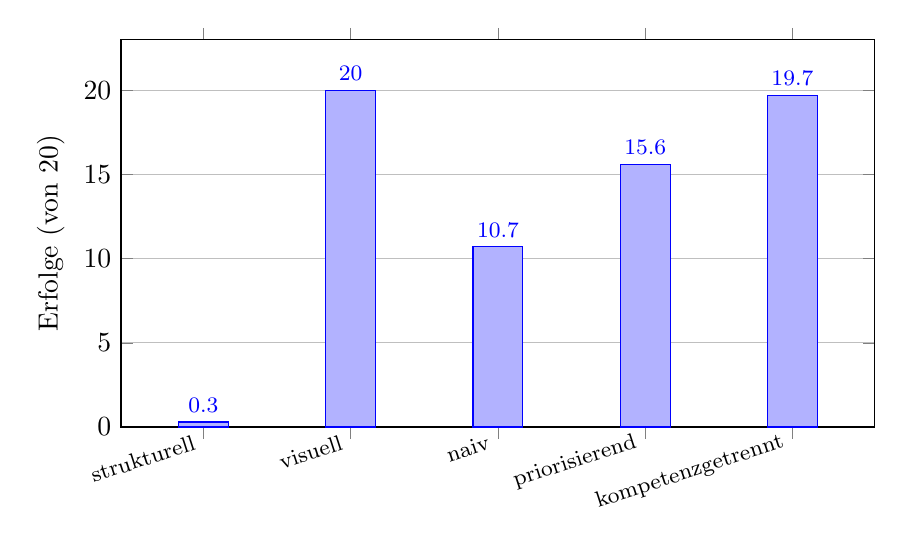
\begin{tikzpicture}
    \begin{axis}[
        ybar,
        width=0.92\linewidth,
        height=6.5cm,
        ymin=0, ymax=23,
        ytick={0,5,10,15,20},
        ylabel={Erfolge (von 20)},
        symbolic x coords={strukturell, visuell, naiv, priorisierend, kompetenzgetrennt},
        xtick=data,
        x tick label style={rotate=18, anchor=east, font=\footnotesize},
        nodes near coords,
        nodes near coords style={font=\footnotesize},
        bar width=18pt,
        enlarge x limits=0.14,
        ymajorgrids=true,
      ]
      \addplot coordinates {(strukturell,0.3) (visuell,20.0) (naiv,10.7) (priorisierend,15.6) (kompetenzgetrennt,19.7)};
    \end{axis}
  \end{tikzpicture}
  \caption{Erfolg in der rein visuellen Kategorie D über die fünf Varianten. Die rein visuelle Variante bildet die Obergrenze, die rein strukturelle scheitert nahezu vollständig. Die naive Kombination erreicht etwa die Hälfte, die Priorisierung verbessert das, und die Kompetenztrennung erreicht nahezu das Niveau der reinen Bildvariante.}
  \label{fig:kategorieD}
\end{figure}

\subsection*{Bewertung}

Gefordert war, dass eine Gestaltung dort belastbar verbessert, wo die naive Kombination scheitert, ohne in den übrigen Kategorien zu verlieren.
Die kompetenzgetrennte Variante erfüllt beides: Sie hebt D1 von 2 auf 29 von 30 Läufen und hält das Niveau in allen anderen gewerteten Kategorien.
Für dieses Szenarioset ist die zweite Forschungsfrage damit positiv beantwortet.
Die beiden Quellen ergänzen sich nicht von selbst, ihr Zusammenspiel lässt sich aber allein über die Instruktion steuern.
Einschränkend kommt hinzu, dass die Variante am Messset entwickelt wurde und Instruktion und Reihenfolge der Schichten nicht getrennt variiert sind; Abschnitt~\ref{sec:eval-validity} führt beides aus.

Als Leitlinie für einen lokalen Agenten mit gemischter Repräsentation lässt sich daraus ableiten, die Quellen nicht nur nebeneinanderzustellen, sondern jeder Schicht den Referenzbereich zuzuweisen, für den sie nach RQ1 exklusiv zuständig ist.
Die visuelle Beschreibung beantwortet dann, welches Objekt gemeint ist, die Struktur, wo es sich befindet.
Da diese Leitlinie auf zwei Szenarien einer Kategorie und einer an diesen Szenarien entwickelten Instruktion beruht, ist sie eine Empfehlung und kein nachgewiesenes Prinzip.
Die kompetenzgetrennte Variante bildet auch die Grundlage des Demonstrators aus Abschnitt~\ref{sec:impl-demonstrator}.


% ------------------------------------------------------------
\section{Validität und Grenzen}
\label{sec:eval-validity}

Die Ergebnisse sind nur so belastbar wie die Kontrolle der Bedingungen, unter denen sie entstanden.
Dieser Abschnitt beschreibt, welche Störfaktoren erkannt und beseitigt wurden, welche Einflüsse bestehen bleiben und wo die Aussagekraft endet.

\subsection*{Beseitigte Störfaktoren und nachträgliche Entscheidungen}

Mehrere zunächst plausible Befunde erwiesen sich bei genauerer Prüfung als Artefakte des Aufbaus und wurden vor der Wertung beseitigt.
Die Farbe der Marker beeinflusste die Farbwahrnehmung des visuellen Modells, das teils die Farbe des Markers statt die des Objekts nannte; die Marker wurden daraufhin versetzt und die Anweisung angepasst.
In Szenarien, in denen ein Referenzobjekt im Koordinatenursprung stand, fielen relative und absolute Zielangabe zusammen, sodass eine relationale Aufgabe auch ohne Verständnis der Relation lösbar war; diese Aufbauten wurden entkonfundiert.
Im ursprünglichen, achsenkollinearen Aufbau von C2 erhielten verdeckte Objekte durch den Sichtbarkeitstest keinen Marker, wodurch das kameranächste Objekt als einziges markiert erschien und die Aufgabe trivial wurde; C2 wurde mit seitlich versetztem Aufbau neu gemessen.
Ein scheinbar deutlicher Nachteil der hybriden Varianten schließlich entpuppte sich als Terminierungsartefakt des Frameworks und verschwand mit dem serverseitigen Schutz gegen identische Wiederholungen (Abschnitt~\ref{sec:impl-agent}).

Dass alle Varianten in der Kontrollkategorie A das Maximum erreichen, zeigt, dass der Messaufbau selbst keine variantenspezifischen Unterschiede erzeugt.
Vollständigkeit lässt sich daraus nicht ableiten: Die genannten Störfaktoren sind die markantesten, nicht notwendigerweise die einzigen.

Einige dieser Eingriffe erfolgten erst, nachdem die zugehörigen Ergebnisse vorlagen.
C3 wurde aus der Auswertung genommen, weil die achsenparallele Kameraausrichtung die aus Sicht der Kamera formulierte Referenz mehrdeutig machte; C2 wurde wegen des oben beschriebenen Markerproblems nicht ausgeschlossen, sondern mit verändertem Aufbau neu gemessen; und E2 wurde als nicht wertbar eingestuft, weil sein Soll-Ergebnis der Grundinstruktion widerspricht, was beim Entwurf nicht bedacht worden war.
In allen drei Fällen lag ein benennbarer Störfaktor vor, nicht bloß ein unerwünschtes Ergebnis.
Vorab festgelegt waren die Entscheidungen aber nicht, und ein solches Vorgehen erhöht grundsätzlich das Risiko, dass die berichtete Auswahl zugunsten der erzählten Deutung ausfällt.

% [INFO BENOETIGT] Ergebnisse der urspruenglichen Fassungen von C2 und C3
% Falls die Messwerte der ersten, spaeter verworfenen Fassungen von C2
% (achsenkollinearer Aufbau) und C3 noch vorliegen, sollten sie im Anhang
% vollstaendig berichtet werden. Das waere der wirksamste Beleg dafuer,
% dass die Ausschluesse sachlich und nicht ergebnisgetrieben erfolgten.
% Falls die Werte nicht mehr vorliegen, bitte hier vermerken, dass die
% Szenarien gemessen wurden, ihre Werte aber nicht erhalten sind.

\subsection*{Abhängigkeit vom Szenarioset}

An zwei Stellen sind die Testfälle in den Aufbau selbst eingeflossen.
Die erste ist der Wahrnehmungs-Prompt (Listing~\ref{lst:vlmprompt}).
Er bestimmt, was die visuelle Schicht überhaupt berichten kann, und begrenzt damit, was sich über ihre Schwächen sagen lässt.
Das Scheitern in B3 geht darauf zurück, dass der Prompt keine Größe abfragt; Kategorie B zeigt deshalb nicht, dass Attributreferenzen grundsätzlich strukturelle Daten erfordern, sondern nur, dass sie es unter diesem Prompt tun.
Umgekehrt nennt der Prompt als Beispiel für einen Texturdeskriptor \enquote{striped}, also das Merkmal, über das D1 und D2 ihr Zielobjekt ansprechen.
Weil alle Varianten mit visueller Schicht denselben Prompt nutzen, verzerrt das den Vergleich \emph{zwischen} ihnen nicht.
Gezeigt ist in Kategorie D aber nur, dass die visuelle Schicht eine Eigenschaft erkennt, auf die ihr Prompt sie ausdrücklich hinweist; ob sie ein unerwartetes Oberflächenmerkmal ebenso zuverlässig berichtet hätte, ist offen.

Die zweite und gewichtigere Stelle betrifft die kompetenzgetrennte Variante.
Sie entstand nicht aus einer vorab formulierten Theorie, sondern aus der Analyse der naiven und der priorisierenden Variante auf demselben Szenarioset, auf dem sie danach gemessen wird, und ihre Instruktion enthält mit \enquote{striped} und \enquote{most salient} zwei Formulierungen aus den Befehlen von D1 und D2 (Listing~\ref{lst:surgical}).
Gezeigt ist damit, dass sich die Kombination beider Schichten auf diesem Set durch die Instruktion erheblich verbessern lässt.
Nicht gezeigt ist, dass die Variante bei ungesehenen Formulierungen ebenso überlegen wäre.
Ein Teil ihres Vorteils könnte darauf beruhen, dass die Instruktion die Wörter des Testbefehls schon enthält und dem Modell die Zuordnung abnimmt, statt eine allgemeine Kompetenz zu vermitteln.
Zwischen beiden Möglichkeiten kann die Arbeit nicht entscheiden; Abschnitt~\ref{sec:zus-ausblick} nennt die Prüfungen, die dafür nötig wären.

\subsection*{Nicht getrennte Einflussgrößen}

Die hybriden Varianten unterscheiden sich nicht nur in ihrer Zuständigkeitsregel.
Die priorisierende stellt zusätzlich die visuelle Beschreibung voran, während die naive und die kompetenzgetrennte mit dem strukturellen Zustand beginnen (Tabelle~\ref{tab:variants}).
Instruktion und Reihenfolge variieren damit gemeinsam, und ihr jeweiliger Beitrag lässt sich nicht trennen.
Für den Vergleich der hybriden Varianten untereinander ist NFA5 insoweit nicht erfüllt; für den Vergleich von strukturell, visuell und hybrid gilt sie, da sich diese Bedingungen in der Repräsentation selbst unterscheiden.

Ungeklärt bleibt auch, warum die naive Kombination den Zugriff auf die visuelle Beschreibung in D1 verliert.
Formulierung des Befehls, visuelle Eindeutigkeit des Zielobjekts und Reihenfolge der Objekte (Abschnitt~\ref{sec:eval-rq2}) sind mit den Daten verträglich und lassen sich in diesem Aufbau nicht voneinander trennen.
Besonders schwer wiegt der Reihenfolgeeffekt, weil er nicht nur den Mechanismus, sondern den Befund selbst betrifft: Das Scheitern der strukturellen Variante mit 0 von 30 passt zu einer Positionspräferenz ebenso gut wie zu einer Verdrängung.
Die Deutung, die exakte strukturelle Information verdränge die unschärfere Beschreibung, ist deshalb eine mögliche Erklärung und kein nachgewiesener Mechanismus.
Die Ähnlichkeit zu Befunden über die Übergewichtung von Text in multimodalen Modellen~\cite{deng2025, wu2025} stützt sie nicht, denn dort konkurrieren Bild und Text innerhalb eines Modells, hier zwei Textquellen (Abschnitt~\ref{sec:grundlagen-sota}).

Ein weiterer Konflikt besteht zwischen der Grundinstruktion und den Mehrobjekt-Szenarien.
Die Grundinstruktion verlangt einen einzigen Manipulationsaufruf, die Soll-Ergebnisse von B2 und E2 betreffen aber mehrere Objekte.
Für E2 macht das die Zelle unwertbar, weil ein Erfolg nur durch Missachtung der Instruktion möglich ist.
Warum B2 den hybriden Varianten trotzdem durchgängig gelingt, ist ungeklärt und hängt davon ab, ob das Löschwerkzeug mehrere Objekte in einem Aufruf annimmt.
Damit bleibt auch offen, ob das knappe Kontextfenster von 4096 Token, das die hybriden Varianten stärker belastet (Abschnitt~\ref{sec:eval-design}), irgendwo wirksam wurde.
Für E2 läge diese Erklärung nahe, B2 spricht aber dagegen, und eine Protokollierung der Kontextauslastung je Lauf, die das klären könnte, wurde nicht vorgenommen.

\subsection*{Messung und Auswertung}

Der Erfolg wird ausschließlich aus dem Folgezustand bestimmt, weil das lokale Modell ein instabiles Abschlussverhalten zeigte.
Es meldete wiederholt Erfolge, die der Folgezustand nicht bestätigte, nannte teils nicht vorhandene Objektkennungen und führte einzelne Manipulationen doppelt aus.
Wie häufig Selbstauskunft und Folgezustand auseinanderfielen, wurde nicht quantifiziert; die Beobachtung beruht auf wiederholten Einzelfällen in den Protokollen.
Für die Gültigkeit der Ergebnisse genügt das, weil ein falsch gemeldeter Erfolg die Erfolgszahl nicht beeinflusst.

Innerhalb einer festen Konfiguration erwies sich die Messung als stabil.
Die meisten Zellen zeigen über die drei Durchläufe eine Spanne von null oder eins, nennenswerte Streuung tritt nur in wenigen Szenarien auf, vor allem in C1 und C4 sowie in D1 und D2 der priorisierenden Variante.
Wie in Abschnitt~\ref{sec:eval-design} ausgeführt, kommt diese Stabilität trotz einer Temperatur von 0{,}8 zustande.
Die Spannen dienen nur noch der Beschreibung der Durchlaufstabilität; die in einer früheren Fassung verwendete Heuristik, nicht überlappende Spannen als belastbaren Unterschied zu werten, wurde durch die Auswertung aus Abschnitt~\ref{sec:eval-metrics} ersetzt.

Die Konfidenzintervalle in Tabelle~\ref{tab:stats} quantifizieren allerdings nur die Unsicherheit innerhalb einer Zelle, nicht die Frage, ob diese Zelle für ihren Referenztyp repräsentativ ist.
Diese zweite Unsicherheit ist die größere und lässt sich hier nicht quantifizieren.
Den bild-exklusiven Bereich belegen zwei Szenarien, den strukturell-exklusiven nach dem Ausschluss von E2 nur eines, und das erlaubt keine Aussage darüber, wie sich der Effekt über die Breite möglicher Referenzen verhält.

Auch die Aufzeichnung der Läufe begrenzt die Analyse.
Für C2 und C4 liegen keine verwertbaren Protokolle mehr vor, sodass sich weder der Lagefehler bestimmen noch nachvollziehen lässt, welches Objekt der Agent in C2 tatsächlich manipuliert hat (Abschnitt~\ref{sec:eval-rq1}).
Werkzeugaufrufe mit Argumenten und erreichte Endpositionen mitzuschreiben, hätte keinen zusätzlichen Messaufwand bedeutet und mehrere der offenen Fragen dieser Arbeit beantwortet; bei einer Wiederholung ist das vorzusehen.
Schließlich wurde nicht geprüft, wie empfindlich insbesondere C2 und C4 auf die Toleranz $\tau = 0{,}1$ reagieren.
Eine großzügigere Toleranz könnte die dortigen Erfolgsraten anheben, ohne dass sich die Rangfolge der Varianten ändern muss.

\subsection*{Technische Einschränkungen}

Die Sichtbarkeitsprüfung arbeitet mit einem einzelnen Sichtstrahl auf den Objektmittelpunkt und kennt nur sichtbar und verdeckt (Abschnitt~\ref{sec:impl-scene}).
Für die verwendeten Szenen genügt das, in dichteren Szenen mit Teilverdeckung nicht.
Der Schutz gegen identische Wiederholungen würde auch eine vom Befehl geforderte Wiederholung blockieren (Abschnitt~\ref{sec:impl-agent}); in den ausgewerteten Szenarien kommt das nicht vor, bei Mehrschritt-Befehlen wäre es aber möglich.

\subsection*{Reichweite}

Alle Befunde beruhen auf einem einzelnen lokalen Modellpaar und auf synthetischen Szenen aus einfachen Grundkörpern.
Innerhalb dieses Rahmens sind sie repliziert und intern konsistent, eine Übertragung auf größere oder anders gebaute Modelle und auf reale, komplexe Szenen wurde aber nicht geprüft.
Für RQ2 kommt hinzu, dass die beste Variante am Szenarioset selbst entwickelt wurde.

Ein Teil der Befunde betrifft eher das Modell als die Repräsentation.
Für C4 ist die Deutung als Präzisionsgrenze tragfähig, denn die Koordinaten liegen vor, die geforderte Rechengenauigkeit wird aber nur manchmal erreicht, und daran ändert keine Repräsentation etwas.
Für C2 ist eine Modellgrenze dagegen nicht belegt (Abschnitt~\ref{sec:eval-rq1}).
C2 enthält zudem mit \enquote{nearest to the camera} eine blickpunktbezogene Referenz; dass blickpunktabhängige Referenzen nicht ausgewertet wurden, gilt also nur für das dafür vorgesehene und ausgeschlossene Szenario C3.

Die Aussagekraft der Arbeit liegt damit in der kontrollierten Isolation der Repräsentationskompetenzen und nicht in einer allgemeinen Gültigkeit über Modelle und Szenen hinweg.

% ============================================================
% KAPITEL 7 — ZUSAMMENFASSUNG UND AUSBLICK
% ============================================================

\chapter{Zusammenfassung und Ausblick}
\label{ch:zusammenfassung}

% ------------------------------------------------------------
\section{Zusammenfassung}
\label{sec:zus-zusammenfassung}

Ausgangspunkt der Arbeit war die Frage, in welcher Form einem lokal betriebenen KI-Agenten eine 3D-Szene bereitgestellt werden sollte, damit er sie über natürliche Sprache manipulieren kann.
Zur Auswahl standen ein struktureller und ein visueller Weg, die beide eigene Stärken haben und jeweils einen Bereich abdecken, den der andere nicht erreicht.

Um diese Frage zu beantworten, wurde ein prototypisches System entwickelt, das dieselbe Szene strukturell, visuell und hybrid bereitstellt und über ein gemeinsames Interface manipulierbar macht.
Die Repräsentationsformen wurden unter gleichen Bedingungen an dreizehn kontrolliert aufgebauten Szenarien verglichen, wobei jede Kombination aus Szenario und Variante in 30 Läufen gemessen und der Erfolg aus dem tatsächlichen Zustand der Szene bestimmt wurde.

Welche Repräsentation am besten abschneidet, hing vom Referenztyp ab, und eine naive Kombination beider Schichten vereinte deren Stärken nicht automatisch.
Erst eine Instruktion, die den Schichten getrennte Zuständigkeiten zuweist, brachte beide auf dem untersuchten Szenarioset zusammen.

Für den Demonstrator wurde diese kompetenzgetrennte Variante in die immersive Zielumgebung übertragen.
Er zeigt, dass die Kette vom Befehl bis zur sichtbaren Manipulation in der Brille funktioniert.
Per Video dokumentiert ist die Fassung mit Bedienmenü, die später ergänzte Spracheingabe nicht.


% ------------------------------------------------------------
\section{Beantwortung der Forschungsfragen}
\label{sec:zus-rq}

\subsection*{Erste Forschungsfrage}

\begin{quote}
\textit{Welchen Einfluss hat die Form der Szenenrepräsentation, strukturell, visuell oder hybrid, auf den Ausführungserfolg der natürlichsprachlichen Szenenmanipulation durch einen lokal betriebenen Agenten, und zwar aufgeschlüsselt nach der Art der sprachlichen Referenz?}
\end{quote}

Für die erste Forschungsfrage lautet das Fazit, dass die Repräsentationsform einen großen Einfluss auf den Ausführungserfolg hat und dieser Einfluss vom Referenztyp abhängt.
Referenzen, deren Merkmal in den Daten kodiert ist, sowie Referenzen auf verdeckte Objekte werden von der strukturellen Form getragen, die als einzige ein im Bild verdecktes Objekt ansprechen kann.
Referenzen auf rein visuelle Eigenschaften wie ein Oberflächenmuster lassen sich nur über die visuelle Form auflösen.

Die naive hybride Form übernimmt den Vorteil der strukturellen Form, den der visuellen nicht zuverlässig.
In der perzeptuellen Kategorie erreicht sie nur 10,7 von 20 möglichen Erfolgen, die visuelle Form alle 20.
Eine Kombination ist also nicht automatisch so gut wie die bessere der beiden Einzelformen.

\subsection*{Zweite Forschungsfrage}

\begin{quote}
\textit{Lässt sich das Zusammenspiel der strukturellen und der visuellen Schicht allein durch die Gestaltung der Instruktion so steuern, dass die hybride Repräsentation die Stärken beider Schichten vereint?}
\end{quote}

Für das untersuchte Szenarioset lässt sich diese Frage mit Ja beantworten, ohne dass die Modelle verändert werden müssen.
Eine Priorisierung einer Schicht reicht dafür nicht, sie verschiebt nur das Gewicht und tauscht eine Kompetenz gegen eine andere.
Eine klare Trennung der Zuständigkeiten, bei der die visuelle Beschreibung das gemeinte Objekt bestimmt und die strukturelle Schicht alle geometrischen Werte liefert, bringt beide Schichten dagegen zusammen.
Die kompetenzgetrennte Variante erreicht so in der perzeptuellen Kategorie 19,7 von 20 und behält gleichzeitig die Stärke der strukturellen Form.


% ------------------------------------------------------------
\section[Beitrag]{Wissenschaftlicher Beitrag}
\label{sec:zus-beitrag}

Inhaltlich zeigt die Arbeit an einem kontrollierten Fall, dass sich strukturelle und visuelle Information nicht automatisch ergänzen.
Ob eine Kombination beide Informationsarten sinnvoll zusammenführt oder ob eine die andere verdrängt, hängt davon ab, wie die Kombination gestaltet ist.
Gewonnen wurde dieser Befund mit einem Modellpaar an dreizehn Szenarien.
Er legt nahe, die Kombination mehrerer Informationsquellen auch bei anderen Agenten als Gestaltungsaufgabe zu sehen und nicht einfach als zusätzliche Information.

Methodisch führt die Arbeit eine nach Referenztypen aufgeschlüsselte Auswertung ein, bei der der Erfolg für jeden Referenztyp einzeln gemessen wird und nicht als ein Gesamtwert.
Erst dadurch werden die exklusiven Zuständigkeiten der Repräsentationen sichtbar, die bei einem pauschalen Vergleich verborgen geblieben wären.
Da dieses Schema nicht an das konkrete System gebunden ist, sollte es sich auch auf ähnliche Vergleiche übertragen lassen.

Praktisch zeigt die Arbeit, dass sich die gesamte Kette aus 3D-Umgebung, Vermittlungsschicht, Agent und zwei gleichzeitig betriebenen lokalen Modellen umsetzen und bis in die immersive Zielumgebung betreiben lässt.


% ------------------------------------------------------------
\section{Ausblick}
\label{sec:zus-ausblick}

Die meisten Ansatzpunkte für weitere Arbeiten ergeben sich direkt aus den Einschränkungen in Abschnitt~\ref{sec:eval-validity}.
Als Erstes sollte geprüft werden, ob die kompetenzgetrennte Variante ihren Vorteil auch außerhalb des Szenariosets behält, auf dem sie entwickelt wurde.
Dafür bräuchte es neue Szenarien, vor allem mit anderen perzeptuellen Eigenschaften als einem Streifenmuster und mit anderen Formulierungen für dieselbe Referenz, sowie eine Fassung der Instruktion ohne \enquote{striped} und \enquote{most salient}, in der die Trennung der Zuständigkeiten rein allgemein formuliert ist.
Erst wenn eine solche Instruktion auch auf neuen Szenarien denselben Vorteil zeigt, ließe sich von einem übertragbaren Gestaltungsprinzip sprechen.

Ähnlich wichtig ist eine Messung, die den Reihenfolgeeffekt in Kategorie D ausschließt.
Dafür würde es reichen, die entscheidenden Szenarien mit vertauschter Objektreihenfolge zu wiederholen und die Reihenfolge der beiden Schichten im Kontext unabhängig von der Instruktion zu verändern.
Beides ist ohne neuen Aufbau möglich.
Bei jeder Wiederholung sollten zudem Werkzeugaufrufe und Endpositionen protokolliert werden, womit sich die offenen Fragen zu C2 und C4 beantworten ließen.

Weitere Ansatzpunkte betreffen die Effizienz und den Umfang des Systems.
Die visuelle Schicht abzurufen dauert spürbar länger als der Abruf des strukturellen Zustands, da ein zusätzlicher Inferenzschritt des Sprach-Bild-Modells nötig ist.
Gemessen wurde dieser Unterschied nicht.
Eine systematische Erhebung von Latenz, Schrittzahl und Rechenaufwand würde diesen bisher nur qualitativ bekannten Trade-off greifbar machen, was vor allem für eine interaktive immersive Anwendung wichtig ist.
Mit steigender Objektzahl dürfte vor allem die visuelle Schicht an ihre Grenzen kommen, weil die Markierung vieler Objekte schnell unübersichtlich wird.
Die Menge der Operationen ließe sich um Drehungen und Skalierungen erweitern sowie um Befehle mit mehreren Manipulationen, deren eigene Schwierigkeiten sich hier bereits angedeutet haben.
Offen sind auch blickpunktabhängige Referenzen, die sich auf die Sicht des Betrachters beziehen und gerade für immersive Umgebungen typisch sind.
Jüngere Arbeiten zur blickpunktabhängigen Segmentierung zeigen, dass solche Bezüge ohne einen expliziten Blickpunkt mehrdeutig sind und von einer ausdrücklichen Darstellung des Blickwinkels profitieren~\cite{nanri2026}.
Eine saubere Behandlung dieses Referenztyps wäre deshalb eine sinnvolle Erweiterung der Taxonomie.

Auf wissenschaftlicher Ebene ließe sich prüfen, ob die gefundenen Kompetenzprofile und die Grenzen der naiven Kombination auch für größere oder anders aufgebaute Modelle gelten oder ob ein größeres Modell das beobachtete Problem von selbst löst.
Ein gezieltes Experiment könnte außerdem die drei offenen Erklärungen voneinander trennen, indem Formulierung, visuelle Eindeutigkeit und Reihenfolge der Objekte unabhängig voneinander verändert werden.
Interessant wäre auch ein Vergleich der zweistufigen Pipeline mit einem einzelnen multimodalen Modell, dem Bild und strukturelle Daten direkt vorliegen.
Damit ließe sich zeigen, ob der beobachtete Effekt von der Pipeline abhängt oder auch unabhängig davon auftritt.
Ob sich das Prinzip der Kompetenztrennung auch auf andere multimodale Aufgaben übertragen lässt, kann Gegenstand zukünftiger Arbeiten werden.

Aus Sicht der Anwendung fehlt noch eine Erprobung mit echten Nutzern.
Die Bewertung in dieser Arbeit ist rein systembasiert, und eine qualitative Nutzerstudie im Demonstrator könnte zeigen, wie Menschen die sprachgesteuerte Manipulation in der immersiven Umgebung tatsächlich erleben.

%----------------------------------------------------------------------
% \backmatter -- Glossar und Literaturverzeichnis
%----------------------------------------------------------------------
\addverzeichnis{Glossar}
\makelexicon
\addverzeichnis{\bibname}
\makebibliography
%----------------------------------------------------------------------
% \appendix -- KI-Nutzungserklaerung und Begleitmaterial gehoeren in den Anhang
%----------------------------------------------------------------------
\appendix
% ============================================================
% KI-Nutzungserklärung (nach OWL-Variante 1)
% Einzufügen NACH dem Literaturverzeichnis / im Anhang.
% Einbindung z. B. via % ============================================================
% KI-Nutzungserklärung (nach OWL-Variante 1)
% Einzufügen NACH dem Literaturverzeichnis / im Anhang.
% Einbindung z. B. via % ============================================================
% KI-Nutzungserklärung (nach OWL-Variante 1)
% Einzufügen NACH dem Literaturverzeichnis / im Anhang.
% Einbindung z. B. via \include{content/ki_erklaerung} im Anhang-Bereich.
% Grundlage: KI-Leitlinie der TH Nürnberg (Amtsblatt 2/2026) und
% OWL-Handreichung "KI-Nutzung in wissenschaftlichen Arbeiten dokumentieren".
% ============================================================

\chapter*{Erklärung: Verwendung von KI-Werkzeugen}
\addcontentsline{toc}{chapter}{Erklärung: Verwendung von KI-Werkzeugen}

Im Rahmen der Erstellung dieser Arbeit wurden generative KI-Werkzeuge eingesetzt.
Die Nutzung wird im Folgenden gemäß der KI-Leitlinie der Technischen Hochschule
Nürnberg Georg Simon Ohm offengelegt.

\begin{itemize}
  \item \textbf{Claude Opus 4.8 (Anthropic):}
        Unterstützung bei der Strukturierung und Gliederung der Arbeit,
        bei der Literaturrecherche mit anschließender Verifikation aller
        Quellen an den Originalpublikationen,
        bei der Erstellung und Überarbeitung von Textentwürfen
        sowie als dialogisches Gegenüber zur Schärfung der Argumentation
        und zur Reflexion des methodischen Vorgehens.
\end{itemize}

Sämtliche von KI-Werkzeugen erzeugten Inhalte wurden eigenständig geprüft,
überarbeitet und inhaltlich verantwortet.
Die Verantwortung für alle Aussagen, Ergebnisse und Schlussfolgerungen dieser
Arbeit liegt vollständig beim Verfasser.
Die reine Rechtschreib- und Grammatikprüfung ist gemäß Leitlinie nicht
dokumentationspflichtig und daher nicht gesondert aufgeführt.

\bigskip
\noindent\textbf{Dokumentationspflichtiger Prompt (inhaltlich prägend).}
Der folgende Prompt trug maßgeblich zur Fundierung der Forschungslücke
(Kapitel~\ref{ch:einleitung} und~\ref{ch:grundlagen}) bei:

\begin{quote}
\enquote{Führe eine wissenschaftliche Literaturrecherche zu Szenenrepräsentationen
für LLM/VLM-Agenten bei natürlichsprachlicher 3D-Szenenmanipulation durch.
Sammle Belege für drei Stränge --- strukturelle, visuelle und hybride
Repräsentation --- sowie für die dazwischen bestehende Forschungslücke,
und schätze ab, wie gut die Lückenbehauptung
(\enquote{ein systematischer, referenztyp-differenzierter Vergleich struktureller,
visueller und hybrider Repräsentation für lokale Agenten fehlt}) gestützt wird.}
\end{quote}

\noindent
Claude Opus 4.8, Anthropic. Die durch die Recherche vorgeschlagenen Quellen
wurden ausnahmslos an den Originalpublikationen überprüft; nicht verifizierbare
Angaben wurden verworfen.
 im Anhang-Bereich.
% Grundlage: KI-Leitlinie der TH Nürnberg (Amtsblatt 2/2026) und
% OWL-Handreichung "KI-Nutzung in wissenschaftlichen Arbeiten dokumentieren".
% ============================================================

\chapter*{Erklärung: Verwendung von KI-Werkzeugen}
\addcontentsline{toc}{chapter}{Erklärung: Verwendung von KI-Werkzeugen}

Im Rahmen der Erstellung dieser Arbeit wurden generative KI-Werkzeuge eingesetzt.
Die Nutzung wird im Folgenden gemäß der KI-Leitlinie der Technischen Hochschule
Nürnberg Georg Simon Ohm offengelegt.

\begin{itemize}
  \item \textbf{Claude Opus 4.8 (Anthropic):}
        Unterstützung bei der Strukturierung und Gliederung der Arbeit,
        bei der Literaturrecherche mit anschließender Verifikation aller
        Quellen an den Originalpublikationen,
        bei der Erstellung und Überarbeitung von Textentwürfen
        sowie als dialogisches Gegenüber zur Schärfung der Argumentation
        und zur Reflexion des methodischen Vorgehens.
\end{itemize}

Sämtliche von KI-Werkzeugen erzeugten Inhalte wurden eigenständig geprüft,
überarbeitet und inhaltlich verantwortet.
Die Verantwortung für alle Aussagen, Ergebnisse und Schlussfolgerungen dieser
Arbeit liegt vollständig beim Verfasser.
Die reine Rechtschreib- und Grammatikprüfung ist gemäß Leitlinie nicht
dokumentationspflichtig und daher nicht gesondert aufgeführt.

\bigskip
\noindent\textbf{Dokumentationspflichtiger Prompt (inhaltlich prägend).}
Der folgende Prompt trug maßgeblich zur Fundierung der Forschungslücke
(Kapitel~\ref{ch:einleitung} und~\ref{ch:grundlagen}) bei:

\begin{quote}
\enquote{Führe eine wissenschaftliche Literaturrecherche zu Szenenrepräsentationen
für LLM/VLM-Agenten bei natürlichsprachlicher 3D-Szenenmanipulation durch.
Sammle Belege für drei Stränge --- strukturelle, visuelle und hybride
Repräsentation --- sowie für die dazwischen bestehende Forschungslücke,
und schätze ab, wie gut die Lückenbehauptung
(\enquote{ein systematischer, referenztyp-differenzierter Vergleich struktureller,
visueller und hybrider Repräsentation für lokale Agenten fehlt}) gestützt wird.}
\end{quote}

\noindent
Claude Opus 4.8, Anthropic. Die durch die Recherche vorgeschlagenen Quellen
wurden ausnahmslos an den Originalpublikationen überprüft; nicht verifizierbare
Angaben wurden verworfen.
 im Anhang-Bereich.
% Grundlage: KI-Leitlinie der TH Nürnberg (Amtsblatt 2/2026) und
% OWL-Handreichung "KI-Nutzung in wissenschaftlichen Arbeiten dokumentieren".
% ============================================================

\chapter*{Erklärung: Verwendung von KI-Werkzeugen}
\addcontentsline{toc}{chapter}{Erklärung: Verwendung von KI-Werkzeugen}

Im Rahmen der Erstellung dieser Arbeit wurden generative KI-Werkzeuge eingesetzt.
Die Nutzung wird im Folgenden gemäß der KI-Leitlinie der Technischen Hochschule
Nürnberg Georg Simon Ohm offengelegt.

\begin{itemize}
  \item \textbf{Claude Opus 4.8 (Anthropic):}
        Unterstützung bei der Strukturierung und Gliederung der Arbeit,
        bei der Literaturrecherche mit anschließender Verifikation aller
        Quellen an den Originalpublikationen,
        bei der Erstellung und Überarbeitung von Textentwürfen
        sowie als dialogisches Gegenüber zur Schärfung der Argumentation
        und zur Reflexion des methodischen Vorgehens.
\end{itemize}

Sämtliche von KI-Werkzeugen erzeugten Inhalte wurden eigenständig geprüft,
überarbeitet und inhaltlich verantwortet.
Die Verantwortung für alle Aussagen, Ergebnisse und Schlussfolgerungen dieser
Arbeit liegt vollständig beim Verfasser.
Die reine Rechtschreib- und Grammatikprüfung ist gemäß Leitlinie nicht
dokumentationspflichtig und daher nicht gesondert aufgeführt.

\bigskip
\noindent\textbf{Dokumentationspflichtiger Prompt (inhaltlich prägend).}
Der folgende Prompt trug maßgeblich zur Fundierung der Forschungslücke
(Kapitel~\ref{ch:einleitung} und~\ref{ch:grundlagen}) bei:

\begin{quote}
\enquote{Führe eine wissenschaftliche Literaturrecherche zu Szenenrepräsentationen
für LLM/VLM-Agenten bei natürlichsprachlicher 3D-Szenenmanipulation durch.
Sammle Belege für drei Stränge --- strukturelle, visuelle und hybride
Repräsentation --- sowie für die dazwischen bestehende Forschungslücke,
und schätze ab, wie gut die Lückenbehauptung
(\enquote{ein systematischer, referenztyp-differenzierter Vergleich struktureller,
visueller und hybrider Repräsentation für lokale Agenten fehlt}) gestützt wird.}
\end{quote}

\noindent
Claude Opus 4.8, Anthropic. Die durch die Recherche vorgeschlagenen Quellen
wurden ausnahmslos an den Originalpublikationen überprüft; nicht verifizierbare
Angaben wurden verworfen.

% ============================================================
% ANHANG A — BEGLEITMATERIAL (Video)
% ------------------------------------------------------------
% ZIELDATEI: content/a1_begleitmaterial.tex
% Einbindung in document.tex NACH \appendix:
%   \appendix
%   % ============================================================
% ANHANG A — BEGLEITMATERIAL (Video)
% ------------------------------------------------------------
% ZIELDATEI: content/a1_begleitmaterial.tex
% Einbindung in document.tex NACH \appendix:
%   \appendix
%   % ============================================================
% ANHANG A — BEGLEITMATERIAL (Video)
% ------------------------------------------------------------
% ZIELDATEI: content/a1_begleitmaterial.tex
% Einbindung in document.tex NACH \appendix:
%   \appendix
%   \include{content/a1_begleitmaterial}
%
% BENOETIGT: fuer den QR-Code das Paket \usepackage{qrcode} im Preamble.
%   (qrcode ist in TeX Live enthalten, kein externes Tool noetig.)
% PLATZHALTER: [VIDEO-URL] durch die stabile, langfristig erreichbare
%   Adresse ersetzen (Uni-Cloud/Repository). Denselben Wert an BEIDEN
%   Stellen eintragen (Text-Link und \qrcode{...}).
% ============================================================

\chapter{Begleitmaterial}
\label{anh:begleitmaterial}

\section{Demonstrationsvideo}
\label{anh:video}

Als Begleitmaterial zu dieser Arbeit steht eine Videoaufzeichnung des Demonstrators zur Verfügung.
Sie zeigt eine frühe Ausbaustufe, in der die Szene über ein Menü in der virtuellen Umgebung manipuliert wird, das vordefinierte Befehle bereitstellt.
Das Video ist unter der folgenden Adresse abrufbar.

\begin{center}
\url{https://git.informatik.fh-nuernberg.de/jobboerse/forschung/bachelorarbeiten/bachelorarbeit-sandro-jaeger/-/blob/fe68f112f06df9da38eff687fd8df8460061186c/BA_VR_Demo_with_menu.mp4}

\vspace{1em}
\qrcode[height=3cm]{https://git.informatik.fh-nuernberg.de/jobboerse/forschung/bachelorarbeiten/bachelorarbeit-sandro-jaeger/-/blob/fe68f112f06df9da38eff687fd8df8460061186c/BA_VR_Demo_with_menu.mp4}

\vspace{0.5em}
{\footnotesize Abbildung: QR-Code zur Videoaufzeichnung.}
\end{center}
%
% BENOETIGT: fuer den QR-Code das Paket \usepackage{qrcode} im Preamble.
%   (qrcode ist in TeX Live enthalten, kein externes Tool noetig.)
% PLATZHALTER: [VIDEO-URL] durch die stabile, langfristig erreichbare
%   Adresse ersetzen (Uni-Cloud/Repository). Denselben Wert an BEIDEN
%   Stellen eintragen (Text-Link und \qrcode{...}).
% ============================================================

\chapter{Begleitmaterial}
\label{anh:begleitmaterial}

\section{Demonstrationsvideo}
\label{anh:video}

Als Begleitmaterial zu dieser Arbeit steht eine Videoaufzeichnung des Demonstrators zur Verfügung.
Sie zeigt eine frühe Ausbaustufe, in der die Szene über ein Menü in der virtuellen Umgebung manipuliert wird, das vordefinierte Befehle bereitstellt.
Das Video ist unter der folgenden Adresse abrufbar.

\begin{center}
\url{https://git.informatik.fh-nuernberg.de/jobboerse/forschung/bachelorarbeiten/bachelorarbeit-sandro-jaeger/-/blob/fe68f112f06df9da38eff687fd8df8460061186c/BA_VR_Demo_with_menu.mp4}

\vspace{1em}
\qrcode[height=3cm]{https://git.informatik.fh-nuernberg.de/jobboerse/forschung/bachelorarbeiten/bachelorarbeit-sandro-jaeger/-/blob/fe68f112f06df9da38eff687fd8df8460061186c/BA_VR_Demo_with_menu.mp4}

\vspace{0.5em}
{\footnotesize Abbildung: QR-Code zur Videoaufzeichnung.}
\end{center}
%
% BENOETIGT: fuer den QR-Code das Paket \usepackage{qrcode} im Preamble.
%   (qrcode ist in TeX Live enthalten, kein externes Tool noetig.)
% PLATZHALTER: [VIDEO-URL] durch die stabile, langfristig erreichbare
%   Adresse ersetzen (Uni-Cloud/Repository). Denselben Wert an BEIDEN
%   Stellen eintragen (Text-Link und \qrcode{...}).
% ============================================================

\chapter{Begleitmaterial}
\label{anh:begleitmaterial}

\section{Demonstrationsvideo}
\label{anh:video}

Als Begleitmaterial zu dieser Arbeit steht eine Videoaufzeichnung des Demonstrators zur Verfügung.
Sie zeigt eine frühe Ausbaustufe, in der die Szene über ein Menü in der virtuellen Umgebung manipuliert wird, das vordefinierte Befehle bereitstellt.
Das Video ist unter der folgenden Adresse abrufbar.

\begin{center}
\url{https://git.informatik.fh-nuernberg.de/jobboerse/forschung/bachelorarbeiten/bachelorarbeit-sandro-jaeger/-/blob/fe68f112f06df9da38eff687fd8df8460061186c/BA_VR_Demo_with_menu.mp4}

\vspace{1em}
\qrcode[height=3cm]{https://git.informatik.fh-nuernberg.de/jobboerse/forschung/bachelorarbeiten/bachelorarbeit-sandro-jaeger/-/blob/fe68f112f06df9da38eff687fd8df8460061186c/BA_VR_Demo_with_menu.mp4}

\vspace{0.5em}
{\footnotesize Abbildung: QR-Code zur Videoaufzeichnung.}
\end{center}
\end{document}